%%%%%%%% ICML 2025 EXAMPLE LATEX SUBMISSION FILE %%%%%%%%%%%%%%%%%

\documentclass{article}

% Recommended, but optional, packages for figures and better typesetting:
\usepackage{microtype}
\usepackage{graphicx}
\usepackage{subfigure}
\usepackage{booktabs} % for professional tables


\usepackage[utf8]{inputenc} % allow utf-8 input
\usepackage[T1]{fontenc}    % use 8-bit T1 fonts
\usepackage{url}            % simple URL typesetting
\usepackage{booktabs}       % professional-quality tables
\usepackage{amsfonts}       % blackboard math symbols
\usepackage{nicefrac}       % compact symbols for 1/2, etc.
\usepackage{microtype}      % microtypography
\usepackage{diagbox}        % For diagonal lines in table cells
\usepackage{makecell}
\usepackage{xspace}
\usepackage{url}
\usepackage{graphicx}
\usepackage{bm}
\usepackage{amssymb}
\usepackage{amsmath}
\usepackage{amsthm}
\usepackage{times}
% \usepackage[ruled,vlined]{algorithm2e}
\usepackage[table,xcdraw]{xcolor}
\usepackage[title]{appendix}
\usepackage{wrapfig}
% \usepackage{hyperref}
\definecolor{customblue}{rgb}{0.36, 0.55, 0.75}
\usepackage[colorlinks=true,linkcolor=magenta, urlcolor=magenta,citecolor=customblue, anchorcolor=magenta]{hyperref}
% \hypersetup{colorlinks=true,linkcolor=blue, urlcolor=magenta,citecolor=blue, anchorcolor=blue}
\usepackage{comment}
\usepackage{bbm}
\usepackage{multirow}
\usepackage{float}
\usepackage{subcaption}
\usepackage{makecell}
\usepackage{verbatim}
\usepackage{enumitem}

\newcommand{\fix}{\marginpar{FIX}}
\newcommand{\new}{\marginpar{NEW}}
\newcommand{\xiang}[1]{{\color{blue}[[Xiang:#1]]}}
\newcommand{\revise}[1]{{\color{blue}#1}}

\urlstyle{same}

\newcommand{\ie}{\textit{i.e.}}
\newcommand{\eg}{\textit{e.g.}}
\newcommand{\etal}{\textit{et al.}\xspace}
\newcommand{\cut}[1]{}
\newcommand{\std}[1]{\scriptsize{$\pm$#1}}
\newcommand{\xhdr}[1]{\vspace{-1mm}\noindent{{\bf #1.}}}
\newcommand{\xhdrnm}[1]{\noindent{{\bf #1.}}}

% \newcommand{\CITE}{{\textcolor{red}{[CITE]}}}

\newcommand{\name}{\textbf{LEAD}\xspace}


\newcommand{\define}[1]{\vspace{0mm}\noindent{{\textbf{#1.}}}}

\usepackage[font=small,labelfont=bf]{caption}
\newcommand{\Hquad}{\hspace{0.3em}}

\usepackage{array}
\newcolumntype{H}{>{\setbox0=\hbox\bgroup}c<{\egroup}@{}}


\usepackage{contour}
\usepackage{ulem}
\renewcommand{\ULdepth}{1.8pt}
\contourlength{0.8pt}
\newcommand{\myuline}[1]{%
  \uline{\phantom{#1}}%
  \llap{\contour{white}{#1}}%
}
\renewcommand{\underline}{\myuline}


\newcommand{\yihe}[1]{{\color{blue}[[yihe: #1]]}}

% hyperref makes hyperlinks in the resulting PDF.
% If your build breaks (sometimes temporarily if a hyperlink spans a page)
% please comment out the following usepackage line and replace
% \usepackage{icml2025} with \usepackage[nohyperref]{icml2025} above.
% \usepackage{hyperref}


% Attempt to make hyperref and algorithmic work together better:
\newcommand{\theHalgorithm}{\arabic{algorithm}}
\usepackage{algorithmic}
\usepackage{listings}
\usepackage{xcolor}
\usepackage{graphicx}
\usepackage{amsmath}
\usepackage{courier}
\usepackage{setspace}


% Use the following line for the initial blind version submitted for review:
% \usepackage{icml2025}

% If accepted, instead use the following line for the camera-ready submission:
\usepackage[accepted]{icml2025}

% For theorems and such
\usepackage{amsmath}
\usepackage{amssymb}
\usepackage{mathtools}
\usepackage{amsthm}

% if you use cleveref..
\usepackage[capitalize,noabbrev]{cleveref}

%%%%%%%%%%%%%%%%%%%%%%%%%%%%%%%%
% THEOREMS
%%%%%%%%%%%%%%%%%%%%%%%%%%%%%%%%
\theoremstyle{plain}
\newtheorem{theorem}{Theorem}[section]
\newtheorem{proposition}[theorem]{Proposition}
\newtheorem{lemma}[theorem]{Lemma}
\newtheorem{corollary}[theorem]{Corollary}
\theoremstyle{definition}
\newtheorem{definition}[theorem]{Definition}
\newtheorem{assumption}[theorem]{Assumption}
\theoremstyle{remark}
\newtheorem{remark}[theorem]{Remark}

% Todonotes is useful during development; simply uncomment the next line
%    and comment out the line below the next line to turn off comments
%\usepackage[disable,textsize=tiny]{todonotes}
\usepackage[textsize=tiny]{todonotes}


% The \icmltitle you define below is probably too long as a header.
% Therefore, a short form for the running title is supplied here:
\icmltitlerunning{LEAD: Foundation Model for EEG-AD}

\begin{document}

\twocolumn[
\icmltitle{LEAD: Large Foundation Model for EEG-Based Alzheimer’s Disease Detection}

% It is OKAY to include author information, even for blind
% submissions: the style file will automatically remove it for you
% unless you've provided the [accepted] option to the icml2025
% package.

% List of affiliations: The first argument should be a (short)
% identifier you will use later to specify author affiliations
% Academic affiliations should list Department, University, City, Region, Country
% Industry affiliations should list Company, City, Region, Country

% You can specify symbols, otherwise they are numbered in order.
% Ideally, you should not use this facility. Affiliations will be numbered
% in order of appearance and this is the preferred way.
\icmlsetsymbol{equal}{*}

\begin{icmlauthorlist}
\icmlauthor{Yihe Wang}{yyy}
\icmlauthor{Nan Huang}{yyy}
\icmlauthor{Nadia Mammone}{zzz}
\icmlauthor{Marco Cecchi}{comp}
\icmlauthor{Xiang Zhang}{yyy}

% \icmlauthor{Firstname4 Lastname4}{sch}
% \icmlauthor{Firstname5 Lastname5}{yyy}
% \icmlauthor{Firstname6 Lastname6}{sch,yyy,comp}
% \icmlauthor{Firstname7 Lastname7}{comp}
%\icmlauthor{}{sch}
% \icmlauthor{Firstname8 Lastname8}{sch}
% \icmlauthor{Firstname8 Lastname8}{yyy,comp}
%\icmlauthor{}{sch}
%\icmlauthor{}{sch}
\end{icmlauthorlist}

\icmlaffiliation{yyy}{Department of Computer Science, University of North Carolina at Charlotte, United States}
\icmlaffiliation{zzz}{DICEAM Department, University Mediterranea of Reggio Calabria, Italy}
\icmlaffiliation{comp}{Cognision, Kentucky, United States}
% \icmlaffiliation{sch}{School of ZZZ, Institute of WWW, Location, Country}

% \icmlcorrespondingauthor{Firstname1 Lastname1}{first1.last1@xxx.edu}
\icmlcorrespondingauthor{Xiang Zhang}{xiang.zhang@charlotte.edu}

% You may provide any keywords that you
% find helpful for describing your paper; these are used to populate
% the "keywords" metadata in the PDF but will not be shown in the document
\icmlkeywords{Machine Learning, ICML}

\vskip 0.3in
]

% this must go after the closing bracket ] following \twocolumn[ ...

% This command actually creates the footnote in the first column
% listing the affiliations and the copyright notice.
% The command takes one argument, which is text to display at the start of the footnote.
% The \icmlEqualContribution command is standard text for equal contribution.
% Remove it (just {}) if you do not need this facility.

\printAffiliationsAndNotice{}  % leave blank if no need to mention equal contribution
% \printAffiliationsAndNotice{\icmlEqualContribution} % otherwise use the standard text.

\begin{abstract}
Hypergraphs provide a superior modeling framework for representing complex multidimensional relationships in the context of real-world interactions that often occur in groups, overcoming the limitations of traditional homogeneous graphs. However, there have been few studies on hypergraph-based contrastive learning, and existing graph-based contrastive learning methods have not been able to fully exploit the high-order correlation information in hypergraphs. Here, we propose a Hypergraph Fine-grained contrastive learning (HyFi) method designed to exploit the complex high-dimensional information inherent in hypergraphs. While avoiding traditional graph augmentation methods that corrupt the hypergraph topology, the proposed method provides a simple and efficient learning augmentation function by adding noise to node features. Furthermore, we expands beyond the traditional dichotomous relationship between positive and negative samples in contrastive learning by introducing a new relationship of weak positives. It demonstrates the importance of fine-graining positive samples in contrastive learning. Therefore, HyFi is able to produce high-quality embeddings, and outperforms both supervised and unsupervised baselines in average rank on node classification across 10 datasets. Our approach effectively exploits high-dimensional hypergraph information, shows significant improvement over existing graph-based contrastive learning methods, and is efficient in terms of training speed and GPU memory cost. The source code is available at \url{https://github.com/Noverse0/HyFi.git}.


% 하이퍼그래프는 집단에서 자주 발생하는 실제 상호작용의 맥락에서 복잡한 다차원 관계를 표현하는 데 탁월한 모델링 프레임워크를 제공하여 기존의 동질적인 그래프의 한계를 극복할 수 있습니다. 하지만 하이퍼그래프 기반 대조 학습과 관련된 연구는 많지 않으며, 기존의 그래프 기반 대조 학습 방법은 하이퍼그래프의 고차 상관관계 정보를 충분히 활용하지 못했습니다. 여기서는 하이퍼그래프에 내재된 복잡한 고차원 정보를 활용하기 위해 고안된 세분화된 하이퍼그래프 대비 학습(FG-HGCL) 방법을 소개합니다. 제안된 방법은 하이퍼그래프 토폴로지를 손상시키는 기존의 그래프 증강 방법을 피하면서 노드 특징에 노이즈를 추가하여 간단하고 효율적인 학습 증강 기능을 제공합니다. 또한 공유 하이퍼에지와 공유 노드를 동질성의 지표로 사용하는 독특한 대비 학습 방식을 사용합니다. 이 방법은 쌍을 이루는 노드 관계를 4개의 세분으로 효율적으로 분류하고 고품질 임베딩을 생성하며 10개의 데이터 세트에서 노드 분류 및 클러스터링 작업에서 감독 및 비감독 기준선보다 뛰어난 성능을 보입니다. 이 접근 방식은 고차원 하이퍼그래프 정보를 효과적으로 활용하여 기존의 그래프 기반 대비 학습 방법에 비해 상당한 개선을 보여주며, 훈련 속도와 GPU 메모리 비용 측면에서 효율적입니다. 소스 코드는 https://github.com/Noverse0/FG-HGCL.git 에서 확인할 수 있습니다.

\end{abstract}

\section{Introduction}
\label{sec:introduction}
% Scientific document retrieval, lack of training data
Scientific document retrieval is a fundamental task that accelerates scientific innovations and access to technical solutions \cite{taxoindex}.
Recently, pre-trained language models (PLMs) have largely enhanced various ad-hoc searches \cite{CTR, DPR}. 
PLM-based retrievers are initially pre-trained on massive textual corpora to develop language understanding.
They are then fine-tuned using vast datasets of annotated query-document pairs, enabling the models to accurately assess the relevance between queries and documents.
However, in specialized domains like scientific document retrieval, constructing large-scale annotated datasets is challenging due to the need for domain expertise \cite{li2023sailer, ToTER, inpars}.
While there are a few general domain datasets (e.g., web search \cite{msmarco_data, NQ_data}), they often fail to generalize to specialized domains \cite{BEIR, inpars}.
This remains a major obstacle~for~applications.


\begin{figure}[t]
    \centering    
    \hspace{-0.2cm}
    \includegraphics[width=0.9\linewidth]{images/intro.pdf}
    \caption{A conceptual comparison of (a) the existing approach for query set generation and (b) our concept coverage-based query set generation. Best viewed in color.}
    \label{fig:intro}
    % \vspace{-0.4cm}
\end{figure}
%% 

% recent solution: synthetic query generation by LLMs
Recently, large language models (LLMs) \cite{GPT3, FLAN, Tzero, Llama} have been actively utilized to generate synthetic data.
Given a document and a prompt including an instruction such as ``\textit{generate five relevant queries to the document}'' \cite{synthetic_apple_VA, dai2022promptagator}, LLMs generate synthetic queries for each document (Figure \ref{fig:intro}a).
The generated queries serve as proxies for actual user queries.
Recent developments in prompting schemes have largely improved the quality of these queries. 
\cite{inpars, dai2022promptagator} show that incorporating a few examples of actual query-document pairs in the prompt leads to the generation of queries with similar distributions (e.g., expression styles) to actual queries.
The state-of-the-art method \cite{pairwise_qgen} employs a \textit{pair-wise} generation that instructs LLMs to generate relevant queries first and then relatively less relevant ones. 
% The generation of irrelevant queries is conditioned on the relevant ones, facilitating the generation of thematically similar rather than completely unrelated queries.
These less relevant queries serve as natural `hard negatives', further improving the efficacy of fine-tuning \cite{pairwise_qgen}.



% Though effective in generating plausible queries, the existing methods impose no conditions for the contents of generation, which often leads to limited coverage of the academic concepts in the document.




\begin{table}[t]
    \caption{An example of synthetic queries. 
    The queries are generated sequentially from $q^1$ to $q^3$. 
    \proposed is applied after generating $q^1$.
    % Repeated concepts are denoted in red, while newly covered concepts are denoted in blue. 
    Repeated keywords are denoted in \textcolor{red}{\textbf{red}}, while newly covered concepts are denoted in \textcolor{blue}{\textbf{blue}}. 
    Details of the generation process are illustrated in Figure \ref{fig:method}.
    % A detailed setup is provided in \cref{sec:experimentsetup}.
    }\small
    \centering
    \renewcommand{\arraystretch}{0.75}
    \resizebox{1\linewidth}{!}{
    \begin{tabular}{C} \toprule
    \textbf{Document} \\ \midrule
     Automated music playlist generation is a specific form of music recommendation. 
     Collaborative filtering methods can be used to ... 
     % Generally stated, the user receives a set of song suggestions ...  
     However, the scarcity of thoroughly curated playlists and the bias towards popular songs ... we propose an alternative model based on a song-to-playlist classifier, ... while leveraging song features derived from audio, ... robust performance when recommending rare and out-of-set songs. ...
     \\ \midrule
     \textbf{Generated queries for the document} \\ \midrule
    \begin{enumerate}[leftmargin=*, after={\vspace*{-0.7\baselineskip}}]% \vspace{-\topsep}
         \item[$q^1$] How can \textcolor{black}{song-to-playlist classifiers} enhance \textcolor{black}{automated music playlist generation}?  
         \item[$q^{2}$] How can \textcolor{red}{automated playlist creation} be boosted through \textcolor{red}{song-to-playlist classification} and \textcolor{blue}{\textbf{feature exploitation}}?  $\,$ (\textit{w/o any condition})
         \item[$q^3$] How does \textcolor{red}{song-to-playlist classifier} differ from traditional \textcolor{blue}{\textbf{collaborative filtering}} for music recommendation? $\quad\,\,\,\,\,\,\,\,\,\,\,$ (\textit{w/o any condition})
    \end{enumerate}\vspace{-\topsep} \\ \hdashline
    \begin{enumerate}[leftmargin=*, after={\vspace*{-\baselineskip}}]  
      \item[$q^{2'}$] What techniques can be used to \textcolor{blue}{\textbf{overcome filter bubbles}} and \textcolor{blue}{\textbf{recommend out-of-set songs}}?  $\quad\quad\quad\quad\quad\quad\quad\quad\quad\quad\quad\quad$ (\textit{w/ \proposed})
     \item[$q^{3'}$] How to \textcolor{blue}{\textbf{leverage mel-spectrogram features}} to \textcolor{blue}{\textbf{mitigate the cold-start problem}} in \textcolor{black}{playlist recommendation}? $\quad\quad\quad\quad\quad\,$(\textit{w/ \proposed})
    \end{enumerate}\vspace{-\topsep} \\ \bottomrule
    \end{tabular}}
    \label{tab:intro}
    \vspace{0.3cm}
\end{table}


% limitation
Though effective in generating plausible queries, the existing methods lack control over the content generated, which can lead to incomplete coverage of the academic concepts in a document.
Academic concepts refer to fundamental ideas, theories, and methodologies that form the contents of scientific documents. 
A scientific document typically explores various concepts.
For example, in Table~\ref{tab:intro}, the document addresses the primary task of music playlist recommendation, along with the design of classification-based models, solutions for popularity biases and data scarcity, and the utilization of audio features.
For a thorough understanding of the document, training queries should comprehensively cover these concepts.


% 

% However, existing methods often generate queries with limited coverage of a document's concepts.
% In the absence of control over the content generated, the queries tend to repeatedly cover similar aspects of the document, leading to high redundancy.
However, in the absence of control over the content generated, the queries often repeatedly cover similar aspects of the document, showing high redundancy.
For example, in Table~\ref{tab:intro}, the generated queries ($q^2, q^3$) repeat keywords such as `automated playlist creation' and `song-to-playlist classification' already present in the previous query ($q^1$).
While these concepts are undoubtedly relevant to the document, such redundant queries cannot effectively bring new training signals.
Furthermore, the queries exhibit a particularly higher lexical overlap with the document, compared to the actual user queries (\cref{result:query_analysis}).
We observe that the queries tend to repeat only a few terms extracted from the document.
Given that users express the same concepts using various expressions in their queries, this limited term usage may not effectively simulate actual queries, reducing the efficacy of fine-tuning.
As a naive solution, one might consider adding more instructions to the prompt, such as ``\textit{use various terms and reduce redundancy among the queries}''.
However, this still lacks systematic control over the generation and fails to bring consistent improvements~(\cref{result:CCQGen});
the improved term usage often appears in common expressions (e.g., advance, enhance, and reinforce), not necessarily enhancing concept coverage.


% While this could be beneficial, a more systematic approach could bring greater effectiveness.


% However, this still lacks systematic control over the generation. and fails to bring consistent improvements~(\cref{result:CCQGen}).
% The improved term usage often appears in common expressions (e.g., ``advance'', ``enhance'', and ``reinforce''), not necessarily enhancing concept coverage and retrieval performance.




We propose \textbf{C}oncept \textbf{C}overage-based \textbf{Q}uery set \textbf{Gen}eration (\proposed) framework to meet two desiderata for training queries: 
(1) The queries should cover complementary aspects, enabling comprehensive coverage of the document's concepts, and (2) The queries should articulate the concepts in various related terms, rather than merely echoing a few phrases from the document.
A key distinction of \proposed is that it adaptively adjusts the generation process based on the concept coverage of previously generated queries (Figure~\ref{fig:intro}b).
% We introduce a \textit{concept extractor} to (1) identify the core concepts of each text and (2) discover strongly related terms not explicitly revealed in the document.
We introduce a \textit{concept extractor} to (1) identify the core concepts of each text and (2) uncover concept-related terms not explicitly mentioned in the document.
Using this information, we discern the concepts not sufficiently covered by previous queries, and leverage them as \textit{conditions} for the subsequent query generation.
Table~\ref{tab:intro} shows that the queries generated with \proposed ($q^{2'}, q^{3'}$) cover complementary concepts using more various~related~terms. 
Furthermore, we introduce new techniques to filter out low-quality queries and enhance retrieval accuracy using the obtained concept information.
Our primary contributions~are:
\begin{itemize}[leftmargin=*]\vspace{-\topsep}
    \item We show that existing query generation methods often fail to comprehensively cover academic concepts in documents, leading to suboptimal training and retrieval performance.
    
    \item We propose \proposed framework, which adaptively imposes conditions for subsequent generation based on the concept coverage.
    \proposed can be flexibly integrated with existing prompting schemes to enhance concept coverage of generated queries.

    \item We validate the effectiveness of \proposed by extensive experiments. 
    \proposed brings significant improvements in query quality and retrieval performance over existing prompting schemes.
    % Furthermore, we provide an in-depth analysis of the \proposed.
\end{itemize}\vspace{-\topsep}




\section{Method}
\label{sec:method}

\begin{figure*}[t]
    \centering
    \includegraphics[width=\linewidth]{figure/deeper.pdf}
    \caption{Framework of \method. Grounded in three high-level goals for direction search, the iterative RL framework progressively enhances the model’s refinement capability through two rounds of self-sampling and training. Applied online in multi-round updates, it enables step-wise persona optimization via directed refinement.}
    \label{fig:deeper}
\end{figure*}


Existing regeneration- and extension-based methods enable dynamic updates but fall short in consistent quality improvement, resulting in a misalignment between the \textit{update step} and the \textit{optimization objective}. To address this, we highlight the critical role of update direction in ensuring effective updates and propose the following core proposition:

\noindent  
\textit{Better update directions lead to better personas.}

\noindent 
Instead of directly searching for improved personas, we optimize refinement directions. By incorporating model predictions into the context and defining three high-level goals for direction search, we propose an iterative reinforcement learning framework with a balanced reward function, enabling effective refinement and continual persona optimization.



\subsection{Refinement Step Formulation}

In \method, each persona refinement step at time $t$, can be formulated as a reinforcement learning (RL) task.
The objective is to learn a policy $\pi_\theta$ to identify optimal refinement directions for specific contexts. For a single user $\mathcal{U}$ in domain $\mathcal{X}$, the refinement step can be formulated as:

\begin{itemize}[noitemsep,left=0pt]
\item \textbf{State:} The previous persona $\mathcal{S}_{t-1}$, generated after the $(t-1)$-th refinement round at the end of the previous window $\mathcal{W}_{t-1}$.

\item \textbf{Observation:} The observation at time step $t$, $\mathcal{O}_t = \{\mathbf{O}_t, \hat{\mathbf{O}}_{t|\mathcal{S}_{t-1}}\}$, where $\mathbf{O}_t$ and $\hat{\mathbf{O}}_{t|\mathcal{S}_{t-1}}$ represent the actual and predicted behaviors in the current window $\mathcal{W}_t$.

\item \textbf{Action:} The refined persona $\mathcal{S}_t$, generated after the $t$-th refinement process based on the corresponding $(\mathcal{S}_{t-1}, \mathcal{O}_t)$ of the user. 

\item \textbf{Policy Model:} The refinement model $\pi_\theta$, maps the state and observation to refined persona $\mathcal{S}_t$:
\vspace{-2mm}
\[
\pi_\theta : (\mathcal{S}_{t-1}, \mathcal{O}_t) \to \mathcal{S}_t. \tag{6}
\vspace{-2mm}
\]
\item \textbf{Reward:} The reward $r_t$ quantifies the effectiveness of the refinement process.
\end{itemize}

\subsection{Direction and Goal Definition}
In this work, we formally define the persona refinement direction and its goals as follows:

\noindent
\paragraph{Definition 3.} (\textit{Persona Refinement Direction}) Identify the directed path of a specific persona refinement step, denoted as $\mathcal{D}_t$, which is uniquely determined by the previous persona $\mathcal{S}_{t-1}$, the current observation $\mathcal{O}_t$, and the refined persona $\mathcal{S}_t$:
\vspace{-2mm}
\[
\mathcal{D}_t \leftrightarrow (\mathcal{S}_{t-1}, \mathcal{O}_t; \mathcal{S}_t). \tag{7}
\vspace{-2mm}
\]


We define three high-level goals for direction search, ensuring comprehensive guidance with temporal insights from past, present, and future.

\noindent
\paragraph{Goal 1.} (\textit{Previous Preservation}): 
Retain stable persona traits from historical behaviors to ensure consistency and preserve critical information.

\noindent
\paragraph{Goal 2.} (\textit{Current Reflection}): Adapt to recent user behaviors by incorporating dynamic changes and correcting errors in the previous persona.

\noindent
\paragraph{Goal 3.} (\textit{Future Advancement}): Enhance the persona’s predictive capability for future behaviors.

\subsection{Reward Function Design}
Given the unique correspondence between $\mathcal{D}_t$ and the triplet $(\mathcal{S}_{t-1}, \mathcal{O}_t; \mathcal{S}_t)$, the quality of $\mathcal{D}_t$ directly determines the refined persona’s quality and process effectiveness within context $(\mathcal{S}_{t-1}, \mathcal{O}_t)$. Accordingly, we formalize three goals of \textit{Direction Quality} as reductions in prediction error from refinement across past, current, and future windows, represented by rewards $r_t^{prev}$, $r_t^{curr}$, and $r_t^{fut}$.

\vspace{-2mm}
\[
r_t^{prev} = \varepsilon_{t-1|\mathcal{S}_{t-1}} - \varepsilon_{t-1|\mathcal{S}_t}
\vspace{-2mm}
\]
\[
r_t^{curr} = \varepsilon_{t|\mathcal{S}_{t-1}} - \varepsilon_{t|\mathcal{S}_t}
\vspace{-2mm}
\]
\[
r_t^{fut} = \varepsilon_{t+1|\mathcal{S}_{t-1}} - \varepsilon_{t+1|\mathcal{S}_t}. \tag{8}
\]

\noindent
$\varepsilon_{t-1|\mathcal{S}_{t-1}}$, $\varepsilon_{t|\mathcal{S}_{t-1}}$, and $\varepsilon_{t+1|\mathcal{S}_{t-1}}$ are prediction errors with previous persona $\mathcal{S}_{t-1}$ across $\mathcal{W}_{t-1}$, $\mathcal{W}t$, and $\mathcal{W}_{t+1}$, respectively, while $\varepsilon_{t-1|\mathcal{S}_t}$, $\varepsilon_{t|\mathcal{S}_t}$, and $\varepsilon_{t+1|\mathcal{S}_t}$ are errors with refined persona $\mathcal{S}_t$.

The total reward for a refinement step is:
\vspace{-2mm}
\[
r_t = r_t^{prev}+ r_t^{curr}+r_t^{fut}. \tag{9}
\]

\subsection{Iterative Training Framework}
\method employs an iterative training framework (Figure~\ref{fig:deeper}): Iteration 1 fine-tunes the base model to refine initial personas (Model 1), while Iteration 2 further enhances it to refine pre-optimized personas (Model 2). Direct Preference Optimization (DPO)\cite{rafailov2024direct} is used to seamlessly integrate rewards into preference pairs, enabling the model to identify better directions through explicit comparisons and supporting scalable iterative fine-tuning.

\paragraph{Iteration 1: Learn to Refine Initial Personas}
Iteration 1 formulates the first refinement step at $t=1$ as an RL task, where we fine-tune the base model to refine initial personas $\mathcal{S}_0$, establishing a baseline policy for direction search and refinement.

\textbf{Context Data Construction}  
First, we initialize personas $\mathcal{S}_0$ for users across multiple domains with their behaviors in window $\mathcal{W}_0$, serving as initial states for refinement processes. The prediction model then predicts user behaviors in $\mathcal{W}_1$ based on $\mathcal{S}_0$. Combining predicted and actual behaviors, we construct observations $\mathcal{O}_1$. Together, $(\mathcal{S}_0, \mathcal{O}_1)$ form the context of the first refinement step.

\textbf{Direction Sampling and Reward Calculation}  
For each context input $(\mathcal{S}_0, \mathcal{O}_1)$, the base model samples $M$ candidate refined personas $\{\mathcal{S}_1^k\}_{k=1}^M$, where each candidate direction $\mathcal{D}_t^k$ is represented by $(\mathcal{S}_0, \mathcal{O}_1; \mathcal{S}_1^k)$. Rewards for these directions as calculated as specified in Equation (9).

\textbf{Preference Pairs Construction and Training}
Refined personas are partitioned into a positive set $\mathcal{S}_1^+$ (rewards $r_t \geq \tau^+$) and a negative set $\mathcal{S}_1^-$ (rewards $r_t \leq \tau^-$) based on reward thresholds. To ensure a clear distinction, we enforce a margin $\delta$, derived from the reward distribution, such that $r_t^w - r_t^l \geq \delta$. The base model is then fine-tuned using DPO with these preference pairs. Following~\cite{gui2024bonbon}, a Supervised Fine-Tuning (SFT) loss is incorporated into the standard DPO objective to maintain alignment with high-quality refinements:
\vspace{-2mm}
\[
\mathcal{L}(\pi_\theta; \pi_{\text{ref}}) = \mathcal{L}_{\text{DPO}}(\pi_\theta; \pi_{\text{ref}}) + \alpha \mathcal{L}_{\text{SFT}}(\pi_\theta). \tag{10}
\]

\paragraph{Iteration 2: Learn to Refine Optimized Personas}
Iteration 2 extends the model's refinement capabilities to handle pre-optimized personas, addressing increased complexity of nuanced refinement tasks.

\textbf{Context Data Construction}
Includes:
(1) Contexts from Iteration 1 $(\mathcal{S}_0, \mathcal{O}_1)$. (2) New contexts $(\mathcal{S}_1, \mathcal{O}_2)$ constructed based on the second refinement step, using $\mathcal{S}_1$ as initial states, with predicted and actual behaviors in $\mathcal{W}_2$ as observations.

\textbf{Direction Sampling and Reward Calculation}
Model 1 is used to sample candidates, following the same procedure of Iteration 1.

\textbf{Preference Pairs Construction and Training}
Similarly to Iteration 1, we construct preference pairs with consistent boundaries for positive and negative sets, with a larger margin $\delta$ to accommodate refined reward distribution and model performance. Model 1 is then fine-tuned with the same combined loss as in Iteration 1, incorporating a subset of preference pairs from Iteration 1 to prevent forgetting and ensure continual learning.








\section{Experiments}
\label{sec:experiments}


\documentclass[border=0pt]{standalone}
\usepackage{pgfplots}
\pgfplotsset{width=\linewidth,compat=1.8}
\usepackage{amsmath}
\usepackage{pgfplotstable}
\usepgfplotslibrary{fillbetween}
\providecommand{\datapath}{.}


\pgfplotsset{every tick label/.append style={font=\boldmath\Huge}}
\tikzstyle{every node}=[font=\bfseries\Huge]

\begin{document}
\pgfplotstableread[col sep=comma,]{\datapath/dcfr9_2.csv}\dcfrb
\pgfplotstableread[col sep=comma,]{\datapath/dcfr16_2.csv}\dcfra
\pgfplotstableread[col sep=comma,]{\datapath/cams_2.csv}\cams
 \LARGE
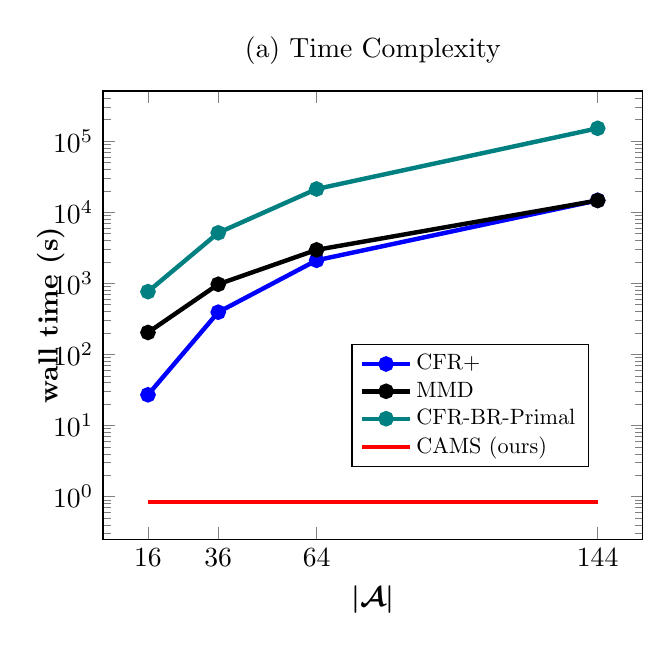
\begin{tikzpicture}[scale=1]
\begin{axis}[title={(a) Time Complexity},
    legend style={nodes={scale=0.8}, style={at={(0.9, 0.435)}}, fill=none},
    legend cell align={left},
    legend entries={CFR+, MMD, CFR-BR-Primal, CAMS (ours)},
    xlabel={$\boldsymbol{|\mathcal{A}|}$},
    ylabel={\textbf{wall time (s)}},
    xtick={16, 36, 64, 144},
    ymode=log,
    % xmode=log,
    ylabel shift=-11pt,
]
% cfr+
\addplot [mark=*, mark size=2pt, ultra thick, blue] coordinates {
(16, 27.05)
(36, 392.77)
(64, 2108.81)
(144, 14707.94)
};
%mmd
\addplot [ultra thick, black, mark=*, mark size=2pt] coordinates {
(16, 203.58)
(36, 970.45)
(64, 2958.36)
(144, 14629.44)
};
%cfr-br-primal
\addplot [ultra thick, teal, mark=*, mark size=2pt] coordinates {
(16, 764)
(36, 5136)
(64, 21238)
(144, 151596)
};
% cams
\addplot [ultra thick, red] coordinates {
(16, 0.842)
(36, 0.842)
(64, 0.842)
(144, 0.842)
};

\end{axis}
\end{tikzpicture}%
% iterations count
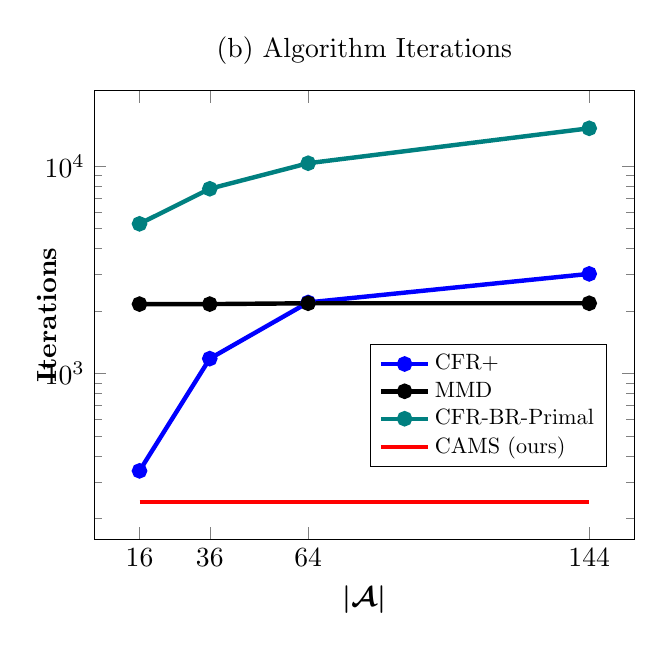
\begin{tikzpicture}[scale=1]
\begin{axis}[title={(b) Algorithm Iterations},
    legend style={nodes={scale=0.8}, style={at={(0.95, 0.435)}}, fill=none},
    legend cell align={left},
    legend entries={CFR+, MMD, CFR-BR-Primal, CAMS (ours)},
    xlabel={$\boldsymbol{|\mathcal{A}|}$},
    ylabel={\textbf{Iterations}},
    xtick={16, 36, 64, 144},
    ymode=log,
    ylabel shift=-11pt,
    % ytick distance=10^.4,
    % log ticks with fixed point,
    % ymin=1e1,
    % ytick={150, 1000, 7000},
    % ytick = {1, 10^1, 10^2, 10^3},
]
% cfr+
\addplot [mark=*, mark size=2pt, ultra thick, blue] coordinates {
(16, 340)
(36, 1180)
(64, 2200)
(144, 3020)
};
%mmd
\addplot [ultra thick, black, mark=*, mark size=2pt] coordinates {
(16, 2160)
(36, 2160)
(64, 2180)
(144, 2180)
};
% cfr-br-primal
\addplot [mark=*, mark size=2pt, ultra thick, teal] coordinates {
(16, 5260)
(36, 7760)
(64, 10300)
(144, 15169)
};
% cams
\addplot [ultra thick, red] coordinates {
(16, 241)
(36, 241)
(64, 241)
(144, 241)
};

\end{axis}
\end{tikzpicture}%
% distance to gt
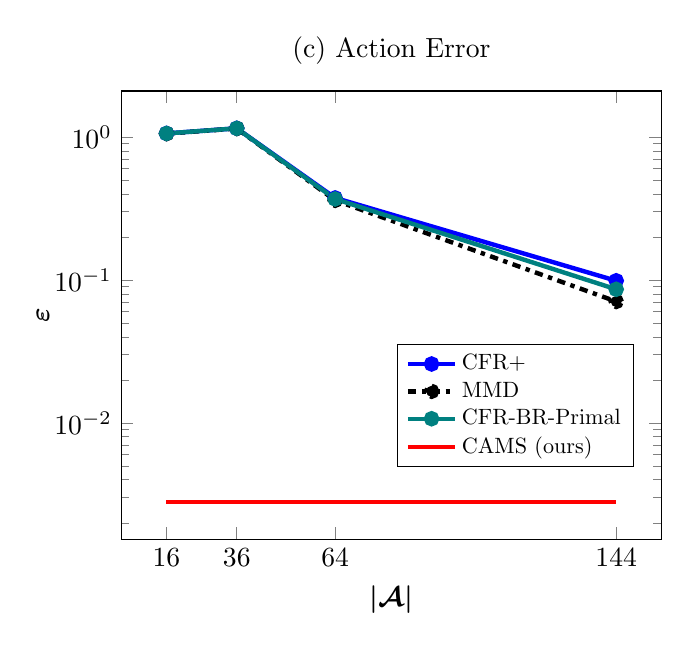
\begin{tikzpicture}[scale=1]
\begin{axis}[title={(c) Action Error},
    legend style={nodes={scale=0.8}, style={at={(0.95, 0.435)}}, fill=none},
    legend cell align={left},
    legend entries={CFR+, MMD, CFR-BR-Primal, CAMS (ours)},
    xlabel={$\boldsymbol{|\mathcal{A}|}$},
    ylabel={$\boldsymbol{\varepsilon}$},
    xtick={16, 36, 64, 144},
    ymode=log,
    ylabel shift=-5pt,
]
% cfr+
\addplot [mark=*, mark size=2pt, ultra thick, blue] coordinates {
(16, 1.0588427800973248)
(36, 1.1494801917079402)
(64, 0.37464195668540257)
(144, 0.09866226893665803)
};
% mmd
% mmd
% [0.5552314866840433,
%  0.5209049957759864,
%  0.5586684894950396,
%  0.6097465051451072]
\addplot[ultra thick, black, mark=*, mark size=2pt, dashdotted] coordinates {
(16, 1.0552507678615948)
(36, 1.146136600348143)
(64, 0.36045590244936615)
(144, 0.07065840307433174)
};
% cfr-br-primal
% 0.6496365514625374,
%  0.2945435474633056,
%  0.1709301707831794,
%  0.03248224069686917
\addplot[ultra thick, mark=*, mark size=2pt, teal] coordinates{
% (16, 0.524)
% (36, 0.568)
% (64, 0.157)
% (144, 0.031)
(16, 1.0581758567678188)
(36, 1.1486716970232314)
(64, 0.3682825954941562)
(144, 0.08599092519673776)
};
% cams
\addplot [ultra thick, red] coordinates {
(16, 0.0028)
(36, 0.0028)
(64, 0.0028)
(144, 0.0028)
};
\end{axis}
\end{tikzpicture}%
\begin{tikzpicture}[scale=1.03]
    \begin{axis}[title={(d) Action Error}, every axis title/.style={above, at={(0.5, 0.986)}},
    legend style={nodes={scale=0.8}, style={at={(0.9, 0.38)}}, fill=none},
    legend cell align={left},
    legend entries={DeepCFR $\boldsymbol{(|\mathcal{A}|=16)}$, DeepCFR $\boldsymbol{(|\mathcal{A}|=9)}$, CAMS (ours)},
    xlabel={$\boldsymbol{t}$},
    ylabel={$\boldsymbol{\bar{\varepsilon}_t}$},
    xtick={0, 0.25, 0.5, 0.75},
    % ytick={0, 5, 10, 15},
    % ymode=log,
    xmax=0.8,
    ylabel shift=-5pt,
]   
% A =16
\addplot [mark=*, mark size=2pt, ultra thick, blue] table[x=x,y=y] {\dcfra};
% A =9
\addplot [mark=*, mark size=2pt, ultra thick, teal] table[x=x,y=y] {\dcfrb};
% cams
\addplot [mark=*, mark size=2pt, ultra thick, red] table[x=x,y=y] {\cams};
% fill betweens
% cfr_9
\addplot [name path=upper,draw=none] table[x=x,y expr=\thisrow{y}+\thisrow{err}] {\dcfrb};
\addplot [name path=lower,draw=none] table[x=x,y expr=\thisrow{y}-\thisrow{err}] {\dcfrb};
\addplot [fill=teal!40, fill opacity=0.4] fill between[of=upper and lower];
% cfr_16
\addplot [name path=upper_2,draw=none] table[x=x,y expr=\thisrow{y}+\thisrow{err}] {\dcfra};
\addplot [name path=lower_2,draw=none] table[x=x,y expr=\thisrow{y}-\thisrow{err}] {\dcfra};
\addplot [fill=blue!40, fill opacity=0.4] fill between[of=upper_2 and lower_2];
% cams
\addplot [name path=upper_3,draw=none] table[x=x,y expr=\thisrow{y}+\thisrow{err}] {\cams};
\addplot [name path=lower_3,draw=none] table[x=x,y expr=\thisrow{y}-\thisrow{err}] {\cams};
\addplot [fill=red!10] fill between[of=upper_3 and lower_3];
    \end{axis}
\end{tikzpicture}
\end{document}



\textbf{Datasets.}
We pre-train on 11 datasets: \textbf{AD-Auditory}~\cite{lahijanian2024auditory}, \textbf{ADFSU}~\cite{vicchietti2023computational}, \textbf{ADSZ}~\cite{pineda2020quantile}, \textbf{APAVA}~\cite{escudero2006analysis}, \textbf{Depression}~\cite{cavanagh2019multiple}, \textbf{PEARL-Neuro}~\cite{dzianok2024pearl}, \textbf{REEG-BACA}~\cite{getzmann2024resting}, \textbf{REEG-PD}~\cite{singh2023evoked}, \textbf{REEG-SRM}~\cite{hatlestad2022bids}, \textbf{TDBrain}~\cite{van2022two}, and \textbf{TUEP}~\cite{veloso2017big}, and fine-tuning on 5 downstream datasets: \textbf{ADFTD}~\cite{miltiadous2023dataset}, \textbf{BrainLat}~\cite{prado2023brainlat}, \textbf{CNBPM}~\cite{amezquita2019novel}, \textbf{Cognision-ERP}~\cite{cecchi2015clinical}, and \textbf{Cognision-rsEEG}. The pre-training datasets include 7 non-AD neurological diseases or healthy subjects and 4 AD datasets, totaling \textit{2,354 subjects and 1,165,361 1-second, 128Hz samples}. All downstream datasets are binary classifications between AD patients and healthy subjects, totaling \textit{615 subjects and 223,039 1-second, 128Hz samples}. The nine AD datasets used for pretraining or fine-tuning consist of \textit{813 subjects} in total. The rationale behind selecting these datasets for pre-training and fine-tuning is discussed in \ref{sub:datasets_selection}. The unified processing pipeline for each dataset is detailed in \ref{sub:data_preprocessing}, with a more detailed description available in Appendix~\ref{sec:datasets_preprocessing}. The statistics for the processed datasets are summarized in Table~\ref{tab:processed_data}.




\textbf{Baselines.}
We compare our method with 10 baselines, including 5 supervised, 3 self-supervised learning, and 2 large EEG foundational models. These selected baselines are state-of-the-art methods or have shown strong performance in EEG or time series classification tasks. The 5 supervised learning methods include \textbf{TCN}~\cite{bai2018empirical}, vanilla \textbf{Transformer}~\cite{vaswani2017attention}, \textbf{Conformer}~\cite{song2022eeg}, \textbf{TimesNet}~\cite{wu2023timesnet}, and \textbf{Medformer}~\cite{wang2024medformer}. The 3 self-supervised learning methods are \textbf{TS2Vec}~\cite{yue2022ts2vec}, \textbf{BIOT}~\cite{yang2024biot}, and \textbf{EEG2Rep}~\cite{mohammadi2024eeg2rep}. The 2 large EEG foundational models are \textbf{LaBraM}~\cite{jiang2024large} and \textbf{EEGPT}~\cite{wangeegpt}. 



\textbf{Implementation.}
All baseline methods and our method's variants, except for LaBraM and EEGPT, are trained under the same code framework. The training epoch for self-supervised pretraining is fixed at 50 epochs, with no early stopping mechanism. The training epoch is set to 100 for fully supervised learning or fine-tuning, with early stopping after 15 epochs of patience based on the best F1 score. The batch sizes for pretraining, fully supervised learning, and fine-tuning are set to 512, 128, and 128, respectively. The optimizer is AdamW. The initial learning rates for pretraining, fully supervised learning, and fine-tuning are set to 0.0002, 0.0001, and 0.0001, respectively, with the CosineAnnealingLR learning scheduler. Gradient norm clipping is set to 4.0, and Stochastic Weight Averaging (SWA)~\cite{izmailov2018averaging} is enabled to benefit inter-subject representation learning. For LaBraM and EEGPT, we use their public code and load their pre-trained model for fine-tuning. We employ four evaluation metrics: sample-level accuracy and F1 score (macro-averaged), and subject-level accuracy and F1 score (macro-averaged) after majority voting, as described in ~\ref{sub:important_setups}. In the self-supervised pre-training stage, all subjects in the datasets are used for training. The ${\lambda_1}$ and ${\lambda_2}$ are both set to 0.5. In the supervised learning or fine-tuning classification stage, the training, validation, and test sets are split based on the subject-independent setup with a ratio of 6:2:2 for each dataset, where each subject appears exclusively in one of these three sets. There is no dataset overlapping between the pre-training and fine-tuning datasets. The training process is conducted with 5 random seeds (41-45) on fixed training, validation, and test sets to compute the mean and standard deviation of the models. All experiments are run on an RTX 4090 GPU and a server with 4 RTX A5000 GPUs, using Python 3.8 and PyTorch 2.0.0 + cu118. Appendix~\ref{sec:implementation_details} provides more details about each method's implementations.




\subsection{Comparison with Baselines}
\label{sub:baseline_comparsion}

\textbf{Setup.} Our method has three variants based on training setups: \textbf{LEAD-Vanilla(3.21M)}, \textbf{LEAD-Sup(3.21M)}, and \textbf{LEAD-Base(3.41M)}. The LEAD-Vanilla model is trained fully supervised on a single dataset without channel alignment, such as the 7-channel version of the Cognision-ERP dataset. LEAD-Sup and LEAD-Base use datasets with alignment to 19 channels. LEAD-Sup is the model trained unified supervised on 5 AD datasets together without pre-training. For LEAD-Base, we first perform self-supervised pre-training on 11 pre-training datasets. The trained model is then used for unified fine-tuning on 5 downstream AD datasets. Note that for both LEAD-Sup and LEAD-Base, the 5 downstream AD datasets are unified trained and evaluated in one run, which is different from the usual approach where supervised training or fine-tuning occurs on a single dataset. The five supervised learning baselines, including TCN, Transformer, Conformer, TimesNet, and Medformer, use the same setup as LEAD-Vanilla. The three self-supervised learning baselines, including TS2Vec, BIOT, and EEG2Rep, follow LEAD-Base's setup. For the two large EEG foundational models, LaBraM and EEGPT, we load their pre-trained models and use the same fine-tuning setup as our LEAD-Base. Appendix~\ref{sec:implementation_details} provides more details about the implementation setups.


\textbf{Results.}
The results are presented in Table~\ref{tab:baseline_comparison}. Our method significantly improves accuracy and F1 score compared with all baselines for both sample-level and subject-level classification. Specifically, our method outperforms the best baseline methods by 6.9\%, 5.72\%, 3.85\%, 7.81\%, and 11.16\% in F1 score at the subject-level on the ADFTD, BrainLat, CNBPM, Cognision-ERP, and Cognision-rsEEG datasets, respectively. The comparison between our method and the supervised learning baselines highlights the effectiveness of channel alignment; although some information might be lost during alignment, the ability to allow unified training still demonstrates substantial performance improvements compared to supervised learning methods on raw-channel datasets. The comparison with self-supervised learning baselines underscores the effectiveness of our contrastive learning approach. The sample-level and subject-level contrasting show a strong learning ability for inter-subject classification. The two large EEG models perform poorly on the ADFTD and BrainLat datasets, achieving almost random results. The comparison between ours and their methods emphasizes the importance of selecting proper pre-training datasets. Our selection of healthy and neurological disease datasets for pre-training contributes significantly to the downstream classification between AD and healthy controls.

Among the three variants of our methods, the LEAD-Base achieves the best performance in most cases, except for the ADFTD dataset, where LEAD-Sup performs better. The comparison between LEAD-Vanilla and LEAD-Sup shows that leveraging more AD datasets for training benefits performance, even in a fully supervised learning manner. The comparison between LEAD-Sup and LEAD-Base indicates that proper self-supervised pre-training methods dramatically reduce the interference of subject features and improve inter-subject classification ability. Besides, We observe that subject-level classification results are typically better than sample-level classification results for almost all methods. This demonstrates that majority voting does alleviate noise interference from outlier samples within a subject. The improvement is particularly notable in the two Cognision datasets. The best performance for these two datasets on the sample-level is around 70\% F1 score, but increases to approximately 90\% with majority voting. Since these datasets were collected in an industrial pipeline with a balanced number of samples per subject (300 or 400), we can infer that the more balanced the number of samples per subject, the greater the improvement introduced by majority voting.






\subsection{Ablation Study and Supplementary Experiments}
\label{sub:ablation_study_supplementary_experiments}
We conduct comprehensive ablation studies, including the effectiveness of non-AD and AD datasets, and contrastive learning modules research, see Appendix~\ref{sec:ablation_studies}. Besides, we conduct additional experiments for more training setups and brain interpretability analysis, including frequency bands analysis and channels analysis. See Appendix~\ref{sec:supplementary_experiments}.








\section{Conclusion}
\label{sec:conclusion}

Tokenizing medical codes is a critical yet challenging step in developing foundation models for electronic health records (EHRs). Existing tokenizers treat medical codes as isolated textual units, failing to capture their structured relationships within large-scale medical ontologies. With more than 600,000 codes that span multiple terminologies, standard tokenization methods struggle to scale while preserving the rich semantic and relational context necessary for downstream clinical and operational tasks.  
%
We introduced \model, a multimodal tokenizer of medical codes that integrates textual definitions and relational ontologies of medical codes to create a unified token representation. \model applies vector quantization to encode both modalities in a structured token space, preserving cross-modality relationships. We integrated \model with five EHR models, evaluating its impact across inpatient (MIMIC-III, MIMIC-IV) and outpatient (EHRShot) settings, as well as in fine-tuning a medical question-answering system.
%
Our results establish \model as a generalizable tokenizer for medical codes, shedding light on how optimizing the tokenization process can benefit medical foundation models.






\clearpage

\section*{Impact Statement}
\label{sec:impact_statement}
This paper introduces the first large foundational model for EEG-based Alzheimer's Disease detection, trained on the largest EEG-AD corpus to date. Our results demonstrate the effectiveness of large pre-trained models and multi-dataset fine-tuning for AD detection, provided that appropriate training methods and datasets are selected. Our approach significantly outperforms methods trained on single datasets and other state-of-the-art self-supervised pre-training methods and large EEG foundational models trained on multiple datasets. The subject-independent evaluation, which tests on unseen subjects, further highlights the applicability of our method in real-world scenarios. We open-source our code, pre-trained model, and fine-tuned model with the hope that this work will drive progress in EEG-based AD detection and inspire future research in detecting other brain disorders and neurodegenerative diseases.


% \section*{Acknowledgement}
% \label{sec:acknowledgement}


\bibliography{refs}
\bibliographystyle{icml2025}


%%%%%%%%%%%%%%%%%%%%%%%%%%%%%%%%%%%%%%%%%%%%%%%%%%%%%%%%%%%%%%%%%%%%%%%%%%%%%%%
%%%%%%%%%%%%%%%%%%%%%%%%%%%%%%%%%%%%%%%%%%%%%%%%%%%%%%%%%%%%%%%%%%%%%%%%%%%%%%%
% APPENDIX
%%%%%%%%%%%%%%%%%%%%%%%%%%%%%%%%%%%%%%%%%%%%%%%%%%%%%%%%%%%%%%%%%%%%%%%%%%%%%%%
%%%%%%%%%%%%%%%%%%%%%%%%%%%%%%%%%%%%%%%%%%%%%%%%%%%%%%%%%%%%%%%%%%%%%%%%%%%%%%%
\clearpage



\appendix
\onecolumn
\setcounter{page}{1}
\begin{appendices}
\newpage
\appendix
\onecolumn

\section*{Appendix}

% \section{Author Contributions}
% \label{sec:ac}
% \begin{itemize}[itemsep=0pt, leftmargin=*]
%     \item Project lead: YB
%     \item Benchmark design: YB, ST, JZ, HP, XW, XL, SC
%     \item Annotation platform: ST, YB
%     \item Annotator recruitment: YB, JX, ST, JZ
%     \item Annotator management: YB, ST, JZ, HP, XL, SC
%     \item Evaluation: YB, assisted by JZ, XL
%     \item Writing: YB, ST, assisted by JZ, HP, XW, XL
%     \item Supervision and fundraising: JL, LH, JT, YD
% \end{itemize}

\section{Model Cards}
Table~\ref{tb:model_card} demonstrates the detailed information of the LLMs and VLMs evaluated in our experiments.

\begin{table}[htbp]
    \centering
    \resizebox{\linewidth}{!}{
    \begin{tabular}{llrr}
    \toprule
    \textbf{Model name} & \textbf{Model version} & \textbf{Context window} & \textbf{Max output tokens} \\
    \midrule
    \emph{Large Language Models}  & \\
    GLM-4-9B-chat~\citep{glm2024chatglm} & - & 128,000 tokens & - \\
    Mistral-Large-Instruct~\citep{jiang2023mistral} & Mistral-Large-Instruct-2407 & 128,000 tokens & - \\
    Deepseek-r1~\cite{guo2025deepseek} & deepseek-reasoner & 64,000 tokens &  8,000 tokens  \\
    \midrule
    \emph{Vison Language Models}  & \\
    MiniCPM-V2.6~\citep{yao2024minicpm} & MiniCPM-V-2-6 & 32,000 tokens & - \\
    % Qwen2-VL-7B~\citep{wang2024qwen2} &  Qwen2-VL-7B-Instruct & 32,000 tokens & - \\
    % Qwen2-VL-72B~\citep{wang2024qwen2} &  Qwen2-VL-72B-Instruct &  32,000 tokens & - \\
     Qwen2.5-VL-7B~\citep{Qwen2.5-VL} &  Qwen2.5-VL-7B-Instruct & 32,000 tokens & - \\
    Qwen2.5-VL-72B~\citep{Qwen2.5-VL} &  Qwen2.5-VL-72B-Instruct &  32,000 tokens & - \\
    Claude 3 Opus~\citep{claude-3} & claude-3-opus-20240229 & 200,000 tokens & 4,096 tokens \\
    % GPT-4V~\citep{achiam2023gpt} & gpt-4-1106-vision-preview & 128,000 tokens & 4,096 tokens	 \\
    Gemini-1.5-pro~\citep{team2024gemini} & gemini-1.5-pro & 2,000,000 tokens & 8,192 tokens	 \\
    GPT-4o~\citep{GPT-4o} & gpt-4o-2024-08-06 & 128,000 tokens & 8,192 tokens \\
    
    \bottomrule
    \end{tabular}
    }
    \caption{Model cards.}
    \label{tb:model_card}
\end{table}



\section{Model Prompts}
\label{sec:task}

\subsection{Prompts for Collecting Visual Instructions}
\xhdr{Prompt for selecting user requests that require 1,000+ word response}
\begin{tcolorbox}[size=title,opacityfill=0.1,breakable]
\noindent
You will receive an image and an instruction from a user to an AI assistant, please determine whether the instruction requires the AI assistant to write an article for the given image, and the length of the article is more than 1,000 words in English (or 1,000 characters in Chinese). If the instruction does not mention the word requirement, please determine whether the user’s intention of the response length is more than 1,000 words. If the instruction is irrelated with the image, please reply “no”.
Instruction: \{\textit{User Instruction}\}
\end{tcolorbox}



\xhdr{Prompt for constructing multi-image instruction}
\begin{tcolorbox}[size=title,opacityfill=0.1,breakable]
\noindent
You will receive {\{\textit{Image Number}\}} images and an instruction from a user to an AI assistant, this original instruction is targeted for the first image solely. Now please rewrite this instruction to a challenging long-output one that need using visual information from all the input images, and the length of the expected output should be more than 2,000 words in English (or 2,000 characters in Chinese). Here are three examples of challenging long-output instructions:

Example instruction 1: \{\textit{Example Instruction 1}\}

Example instruction 2: \{\textit{Example Instruction 2}\}

Example instruction 3: \{\textit{Example Instruction 3}\}

Now, you should rewrite the following instruction:

Instruction: \{\textit{User Instruction }\}

Please rewrite this user instruction to a challenging long-output instruction that requires the use of all the input images. Please output only the rewritten instruction, do not output other content.
\end{tcolorbox}

\subsection{Prompts for the LongWrite Agent-V Pipeline}
\label{app:prompt_lav}

\xhdr{Prompt for planning the writing outline}
\begin{tcolorbox}[size=title,opacityfill=0.1,breakable]
\noindent
You are an expert planner. Your task is to break down a writing task into clear subtasks based on the provided images and writing instruction.

Please analyze the images and writing instruction carefully, then create a detailed outline in this format:

Section 1 - Main Point: [Key points to cover based on images and instruction] - Word Count: [200-1000 words]

Section 2 - Main Point: [Key points to cover based on images and instruction] - Word Count: [200-1000 words]

...

Make each section focused and specific while ensuring the full outline:

1. Covers all key content from both images and writing instruction

2. Flows logically from section to section

3. Has reasonable word count targets (200-1000 words per section)

4. Forms a cohesive whole that fulfills the writing instruction

Writing instruction: \{\textit{User Instruction}\}

Output only the outline with no other text.
\end{tcolorbox}


\xhdr{Prompt for generating each paragraph according to the writing outline}
\begin{tcolorbox}[size=title,opacityfill=0.1,breakable]
\noindent
You are an expert writer. Your task is to write the next section of a longer piece based on:

1. The provided images and writing instruction

2. The outline plan

3. Previously written sections

Writing instruction:  \{\textit{User Instruction}\}

Outline plan: \{\textit{PLAN}\}

Previous sections: \{\textit{TEXT}\}


Please write section  \{\textit{STEP}\} following these guidelines:

1. Focus on the main points specified in the outline

2. Stay within the target word count

3. Flow naturally from previous sections

4. Integrate relevant details from the images

5. Maintain a consistent tone and style

6. Write only this section, not a full conclusion

Output only the new section with no other text.
\end{tcolorbox}


\section{Annotation Details}

\subsection{Annotation Platform}
\label{sec:platform}

Our annotation platform consists of two main pages: annotation page and admin page.

\noindent
\textbf{\rednote{Annotation page.}} 
This page provides the core annotation interface for users. As shown in Figure~\ref{fig:Annotation_Annotation1}, after logging in, users first see a course selection interface where they can view available courses in their major. Each course is displayed with a progress bar showing completion status and the total number of annotated pages. After selecting a course, users enter the annotation interface shown in Figure~\ref{fig:Annotation_Annotation2}, where the page is divided into three columns: the lecture slide, original transcript, and annotation area. Users can navigate through slides using pagination controls and save their annotations for each slide individually.

\noindent
\textbf{\rednote{Admin page.}} 
This page provides administrative oversight of the annotation process. As shown in Figure~\ref{fig:Annotation_Admin1}, administrators can monitor annotation progress across all majors and courses, with detailed statistics grouped by annotator's major. The interface displays progress bars and completion rates for each course, helping administrators track the overall project status. When reviewing annotations, administrators can examine both original and modified scripts side by side, as shown in Figure~\ref{fig:Annotation_Admin2}.

\begin{figure}[t]
    \centering
    \includegraphics[width=\linewidth]{figs/appendix/Annotation_Annotation1.png}
    \caption{Screenshot of the \rednote{annotation page} (course selection). After logging in, annotators can view available courses in their major, with progress bars showing completion status and the number of annotated pages.}
    \label{fig:Annotation_Annotation1}
\end{figure}

\begin{figure*}[htbp]
    \centering
    \includegraphics[width=\linewidth]{figs/appendix/Annotation_Annotation3.png}
    \caption{Screenshot of the \rednote{annotation page} (annotation). The page displays the lecture slide (left), original transcript (middle), and annotation area (right). Users can modify transcripts while viewing the corresponding slides and track their annotation status.}
    \label{fig:Annotation_Annotation2}
\end{figure*}

\begin{figure}[htbp]
    \centering
    \includegraphics[width=\linewidth]{figs/appendix/Annotation_Admin1.png}
    \caption{Screenshot of the \rednote{admin page} (progress overview). Administrators can monitor annotation progress across different majors, view detailed statistics for each course, and track overall completion status.}
    \label{fig:Annotation_Admin1}
\end{figure}

\begin{figure}[htbp]
    \centering
    \includegraphics[width=\linewidth]{figs/appendix/Annotation_Admin3.png}
    \caption{Screenshot of the \rednote{admin page} (review interface). Reviewers can examine both original and modified scripts side by side.}
    \label{fig:Annotation_Admin2}
\end{figure}







\clearpage
\subsection{Annotation Guidelines}
\label{sec:guide}


\noindent
\textbf{\bluenote{\underline{Guidelines for the data annotators:}}}

\begin{tcolorbox}[size=title,opacityfill=0.05,breakable]
\noindent
1. Click on ``Register'' in the left bottom part of the annotation page if this is the first time that you enter our system. You should choose your major, username and password during registration. We will assign annotation tasks according to your major. You can return to the annotation page and login via your username and password.

2. After logging in, you will see a list of PPTs that require modifications to the presentation scripts. Click on “Start Annotating” to proceed.

3. After opening a PPT, you will see the original script for each slide. These scripts are generated by AI and may have issues such as factual errors, missing information from the PPT, irrelevance to the topic, awkward phrasing, or repetitive wording. Your task is to edit the script for each slide in the "Annotation Area." After making your changes, click on "Save Annotations."

4. Note that this is a one-way system. If you press the browser's back button, the login process will restart (there are only three pages: login, list, and annotation). If you want to return to the list page from the annotation page, you can click on "Return to Course List" at the top. Remember to save your annotations promptly after completing them! Click "Save Annotations" immediately after finishing your annotations! If the PPT is not clear enough, you can use the button at the top-right corner of the image to enlarge it to full screen.

5. If you have finished marking a PPT, you can contact us for acceptance inspection. We will check each page for the following:

- Whether there are factual errors.

- Whether too much information from the PPT is missing in the script.

- Whether the content is irrelevant to the topic.

- Whether the sentences are awkward or not smooth.

- Whether there is repetitive wording.

6. Compensation:

- If every page of the PPT passes the acceptance inspection, you will receive a base payment of \texttt{80} \texttt{CNY} for each PPT.

- If a PPT fails the acceptance inspection three or more times, each subsequent failure will result in a deduction of \texttt{20} \texttt{CNY} from the payment, to compensate for the time spent by the inspector.

- If the original script of the PPT is empty on six or more pages, and the PPT passes the acceptance inspection, you will receive an additional \texttt{20} \texttt{CNY} in compensation for the time spent by the annotator in writing the script from scratch.

\textbf{After reading the above requirements, start data annotation now!}

\end{tcolorbox}

\subsection{Data Collection Cost}
We spend approximately \texttt{7,000 CNY} on human correction data collection.

\section{More Evaluation Details}
\label{sec:setup}


\subsection{Evaluation Setting}
In the Image + VLM setting, we set the generation sampling parameters to  \texttt{max\_new\_tokens}=8192. In the Caption + LLM setting, for the first model call where we use gpt-4o for generating the caption, we set \texttt{max\_new\_tokens}=1024. For the following model call where the LLM outputs the final response for the writing instruction and caption, we set \texttt{max\_new\_tokens}=8192 except for claude-3-opus, which we set \texttt{max\_new\_tokens}=4096.

\subsection{Evaluation Prompts}

\xhdr{Prompt for gpt-4o on generating caption for the \textit{Caption + LLM} setting}

\begin{tcolorbox}[size=title,opacityfill=0.05,breakable]
\noindent
Please provide a detailed and comprehensive description of the image, paying special attention to both visual elements and textual content. Consider the following aspects:

1. Main Subject(s):

   - What are the primary objects, people, or figures in the image?
   
   - Their positioning, size, and prominence
   
   - Any diagrams, charts, or graphical elements
   

2. Textual Content:

   - All text visible in the image, including:
   
     * Headers, titles, or captions
     
     * Labels or annotations
     
     * Body text or paragraphs
     
     * Numbers, equations, or mathematical notation
     
   - The relationship between text and visual elements

3. Visual Details:

   - Colors, lighting, and overall composition
   
   - Textures and materials visible
   
   - Any notable patterns, designs, or visual hierarchies
   
   - Quality and clarity of text/figures

4. Information Structure:

   - How information is organized (e.g., flowcharts, tables, lists)
   
   - Connections or relationships indicated by arrows or lines
   
   - Legend or key elements if present
   
   - Reading order or flow of information

5. Technical Elements:

   - Presence of graphs, charts, or scientific figures
   
   - Any coordinate systems or axes
   
   - Units of measurement or scales
   
   - Technical symbols or notation

6. Context and Purpose:

   - The apparent purpose of the image (educational, technical, decorative, etc.)
   
   - Target audience or field of study
   
   - Any relevant domain-specific context

Please provide a clear, structured description that captures both the visual and textual elements, ensuring no significant details are omitted.
\end{tcolorbox}

\xhdr{Prompt for LLMs on generating response for the \textit{Caption + LLM} setting}

\begin{tcolorbox}[size=title,opacityfill=0.05,breakable]
\noindent
Please analyze the following image captions and writing requirement carefully, then provide a detailed response that:

        1. Directly addresses the writing requirement
        
        2. Incorporates relevant details from the image captions
        
        3. Uses clear, well-structured writing
        
        4. Maintains appropriate tone and style for the context

Writing requirement: \{\textit{User Instruction}\}


Image captions: \{\textit{CAPTIONS}\}


Please provide a comprehensive response that fully satisfies the writing requirement while effectively utilizing the information from the image captions.
\end{tcolorbox}

\xhdr{Prompt for gpt-4o on scoring the quality of responses}

\begin{tcolorbox}[size=title,opacityfill=0.05,breakable]
\noindent
You are an expert in evaluating text quality. Please evaluate the quality of an AI assistant's response to a user's writing request with several corresponding images. Be as strict as possible.

You need to evaluate across the following six dimensions, with scores ranging from 1 to 5. The scoring criteria from 5 to 1 for each dimension are as follows:

1. Relevance: From content highly relevant and fully applicable to the user's request and images to completely irrelevant or inapplicable.

2. Accuracy: From content completely accurate with no factual errors or misleading information to content with numerous errors and highly misleading.

3. Coherence: From clear structure with smooth logical connections to disorganized structure with no coherence.

4. Clarity: From clear language, rich in detail, and easy to understand to confusing expression with minimal details.

5. Breadth and Depth: From both broad and deep content with a lot of information to seriously lacking breadth and depth with minimal information.

6. Reading Experience: From excellent reading experience, engaging and easy to understand content to very poor reading experience, boring and hard to understand content.

Please evaluate the quality of the following response to a user's request according to the above requirements.

<User Request>

 \{\textit{INST}\}

</User Request>

<Response>

 \{\textit{RESPONSE}\}

</Response>

Please evaluate the quality of the response. You must first provide a brief analysis of its quality, then give a comprehensive analysis with scores for each dimension. The output must strictly follow the JSON format: {"Analysis": ..., "Relevance": ..., "Accuracy": ..., "Coherence": ..., "Clarity": ..., "Breadth and Depth": ..., "Reading Experience": ...}. You do not need to consider whether the response meets the user's length requirements in your evaluation. Ensure that only one integer between 1 and 5 is output for each dimension score.
\end{tcolorbox}


\subsection{Deployment Details}
All the experiments were conducted on an Ubuntu 20.04.4 server equipped with 104 Intel Xeon(R) Platinum 8470 CPU cores, and graphic cards that contained 8 NVIDIA
A800 SXM 80GB GPUs. Besides, the CUDA version is 12.2. 
The supervised fine-tuning (SFT) phase for LongWriter-V-7B on the LongWrite-V-22k dataset took approximately six hours using 8 GPUs. For the LongWriter-V-72B model, the SFT process required 72 hours with the same GPU configuration. The Direct Preference Optimization (DPO) process for LongWriter-V-7B, using 2,844 mixed preference pairs, completed in 1.5 hours.
% The SFT phase of LongWriter-V-7B on the LongWrite-V-22k data takes about six hours with the 8 GPUs. And the SFT process of LongWriter-V-72B model requires 72 hours with 8 GPUs. For the DPO process on LongWriter-V-7B with 2,844 mixed preference pairs, it takes 1.5 hours to finish.


% \section{Results for Each Subtask}
% \subsection{Performance on Benchmark}
% The evaluation results for each subtask of MMLongBench-Write are shown in Table~\ref{tb:exp_subtask}. 

% \begin{table}[t]
% \centering
% \resizebox{\linewidth}{!}{
% \begin{tabular}{l|cc|cc|cc|cc|cc|cc|cc}
% \toprule
%  &  & & \multicolumn{6}{|c}{\textbf{Professional Writing}} & \multicolumn{6}{|c}{\textbf{Creative Writing}} \\
% \cmidrule(r){1-3} \cmidrule(lr){4-9} \cmidrule(l){10-15}
% \textbf{Model} & \multicolumn{2}{c|}{\textbf{Overall}} & \multicolumn{2}{c|}{\textbf{PPT}} & \multicolumn{2}{c|}{\textbf{Travel}} & \multicolumn{2}{c|}{\textbf{Medical}} & \multicolumn{2}{c|}{\textbf{Story}} & \multicolumn{2}{c|}{\textbf{Scenery}} & \multicolumn{2}{c}{\textbf{Movie}} \\ 
%  & $S_l$ & $S_q$  & $S_l$ & $S_q$  & $S_l$ & $S_q$  & $S_l$ & $S_q$  & $S_l$ & $S_q$  & $S_l$ & $S_q$  & $S_l$ & $S_q$ \\ 
% \midrule
% \multicolumn{12}{l}{\emph{Caption + LLMs}} \\
% \texttt{GLM-4-9B-Chat} & 60.9 & 75.2 & 39.6 & 78.8 & 67.4 & 84.0 & 70.5 & 66.7 & 76.4 & 81.0 & 41.7 & 63.3 & 69.9 & 77.3 \\
% \texttt{GPT-4o-2024-05-13} & 65.8 & 84.8 & 44.9 & 90.4 & 75.3 & 89.0 & 76.8 & 78.3 & 79.8 & 88.3 & 49.8 & 74.0 & 68.3 & 88.8 \\
% \texttt{Mistral-Large-Instruct-2407} & 70.3 & 80.9 & 48.2 & 86.5 & 82.9 & 85.0 & 77.4 & 74.6 & 85.1 & 82.9 & 56.8 & 74.2 & 71.2 & 82.1 \\
% \texttt{DeepSeek-R1} & 71.2 & 86.5 & 56.6 & 89.8 & 90.6 & 92.3 & 74.7 & 80.0 & 89.4 & 89.8 & 61.9 & 77.9 & 53.8 & 89.2 \\
% \midrule
% \multicolumn{12}{l}{\emph{Open-source VLMs}} \\
% \texttt{MiniCPM-V2.6} & 20.4 & 61.4 & 22.4 & 63.1 & 33.2 & 89.6 & 19.3 & 57.5 & 7.2 & 18.1 & 3.7 & 71.0 & 36.7 & 69.2 \\
% \texttt{Qwen2-VL-7B-Instruct} & 39.0 & 63.3 & 33.5 & 56.2 & 19.3 & 82.7 & 41.9 & 35.0 & 69.7 & 66.7 & 32.2 & 72.1 & 37.6 & 66.9 \\
% \texttt{Qwen2-VL-72B-Instruct} & 49.7 & 77.7 & 45.2 & 77.9 & 33.7 & 84.2 & 53.2 & 58.3 & 79.0 & 84.0 & 32.1 & 82.1 & 54.9 & 80.0 \\
% \midrule
% \multicolumn{12}{l}{\emph{Proprietary VLMs}} \\
% \texttt{Claude-3-Opus-20240229} & 42.5 & 77.6 & 30.8 & 72.5 & 52.9 & 91.9 & 35.9 & 64.0 & 49.0 & 72.5 & 42.9 & 85.8 & 43.6 & 79.0 \\
% \texttt{GPT-4o-2024-05-13} & 57.1 & 89.7 & 41.7 & 89.4 & 53.4 & 94.2 & 67.7 & 84.2 & 88.4 & 95.0 & 22.1 & 84.2 & 69.5 & 91.3 \\
% \texttt{GPT-4-1106-vision-preview} & 58.7 & 90.5 & 38.6 & 89.2 & 55.1 & 94.4 & 73.4 & 88.7 & 89.9 & 95.0 & 25.3 & 85.8 & 69.7 & 89.6 \\

% \midrule
% \multicolumn{12}{l}{\emph{Our trained VLMs}} \\
% \texttt{LongWriter-V-7B} & 85.4 & 78.6 & 89.6 & 81.5 & 89.3 & 86.9 & 79.7 & 71.7 & 69.8 & 76.7 & 92.7 & 76.0 & 91.6 & 78.7 \\
% \texttt{LongWriter-V-72B} & 81.6 & 83.7 & 91.1 & 85.8 & 91.9 & 90.2 & 83.2 & 77.1 & 54.5 & 80.2 & 85.7 & 83.3 & 83.3 & 85.6 \\
% \texttt{LongWriter-V-7B-DPO} & 85.8 & 80.7 & 90.4 & 79.6 & 87.8 & 91.2 & 87.2 & 75.4 & 69.8 & 78.8 & 88.2 & 76.5 & 91.3 & 82.9 \\
% \bottomrule
% \end{tabular}
% }
% \caption{Evaluation results (\%) on MMLongBench-Write. Note that the benchmark contains six subtasks: PPT Script, Travel Guide, Medical Report, Story Generation, Scenery Copywriting, Movie Review. We report scores on different subsets of the benchmark, where we use the first word of the task for abbreviation. $\overline{S}$, $S_l$, $S_q$ is the overall score, length score and quality score respectively.}
% \label{tb:exp_subtask}
% \end{table}



% \subsection{Case Study}


\clearpage
\subsection{Case Study}
\label{sec:case}


\begin{figure}[htbp]
    \centering
    \includegraphics[width=\linewidth]{figs/appendix/case.pdf}
    \caption{Input images of the example for the PPT script generation task.}
    \label{fig:input_case}
\end{figure}

% To showcase how the real outputs of our tested models are, we select a case from MMLongBench-Write. As shown in Figrue~\ref{fig:input_case}, there are 15 input images for this case. The instruction of this case is `` Write a 3000-word lecture script based on these ppt images. The script can be read aloud by a teacher in class and should not contain any unreadable content. The script should be consistent with the teaching goal of the ppt and not simply repeat the content on the ppt. It should be clear, structured, and have educational and inspirational value. Please output the script directly, without any extra content like subtitles or questions, and please again ensure that the script is readable. '' We have listed the responses of GPT-4o-2024-08-06, LongWriter-V-72B and LongWriter-V-7B-DPO as following:

To illustrate the actual outputs of our tested models, we select a case from MMLongBench-Write. As shown in Figure~\ref{fig:input_case}, this case includes 15 input images. The instruction for this case is as follows:
``Write a 3000-word lecture script based on these PPT images. The script should be suitable for a teacher to read aloud in class and must not contain any unreadable content. It should align with the teaching goals of the PPT without merely repeating its content. The script should be clear, well-structured, and possess educational and inspirational value. Please output the script directly, without additional content such as subtitles or questions, and ensure it is fully readable.''
We present the responses from GPT-4o-2024-08-06, LongWriter-V-72B, and LongWriter-V-7B-DPO below:

\noindent
\textbf{\bluenote{\underline{Response of GPT-4o-2024-08-06:}}}

\begin{tcolorbox}[size=title,opacityfill=0.05,breakable]
\noindent
Ladies and gentlemen, welcome to today's lecture on Mechanical Energy. Our focus will be on understanding the fundamental concepts of kinetic energy, potential energy, and the roles of air resistance and friction. These concepts are not just theoretical; they have practical implications in our daily lives, especially in the context of transportation.

Let's begin by considering the significance of transportation in energy consumption. In the United States, transportation accounts for approximately 28\% of total energy use, which translates to about 30 exajoules per year. This sector also contributes to one-third of the country's CO2 emissions. Understanding the mechanics behind transportation can help us devise strategies to reduce energy use and emissions.

First, let's delve into kinetic energy, which is the energy of motion. The formula for kinetic energy is \( E_{\text{kin}} = \frac{1}{2}mv^2 \), where \( m \) is mass and \( v \) is velocity. Consider a baseball thrown at 100 mph; its kinetic energy is around 150 joules. While this is a small amount of energy, it illustrates the concept effectively. Now, imagine a car like a Toyota Camry with four passengers moving at 60 mph. The kinetic energy here is approximately 700 kilojoules, demonstrating how energy scales with mass and velocity.

Let's explore a practical example: a road trip from Boston to New York, a distance of 210 miles. Suppose the car in question achieves 30 miles per gallon and consumes 7 gallons of fuel for the trip, equating to 840 megajoules of energy. However, not all this energy is used for motion. The kinetic energy required is only about 0.7 megajoules. So, where does the rest of the energy go? Factors like engine efficiency, air resistance, and friction play significant roles.

Next, we'll explore potential energy, which is stored energy based on an object's position or configuration. A fundamental principle here is energy conservation: energy cannot be created or destroyed, only transformed. Consider a ball rolling uphill; kinetic energy is converted into potential energy. The potential energy, \( U \), is given by \( U = mgh \), where \( g \) is the acceleration due to gravity, and \( h \) is height. Springs are another example, where potential energy is stored as \( U = \frac{1}{2}kx^2 \).

Now, let's consider potential energy in the context of forces and work. For a mass subject to a force, the work done is the force multiplied by the distance moved. This work results in energy transfer, such as converting potential energy to kinetic energy. In vector terms, for motion in a line, force is related to potential energy by \( F = -\frac{dU}{dx} \).

Let's apply these concepts to real-world scenarios. Consider an airplane cruising at altitude; its kinetic energy is significant. But potential energy also plays a crucial role, especially at high altitudes. Other applications include using potential energy to pump water uphill or using elevators and cranes.

Returning to our road trip example, we must consider the potential energy effects of hills. A constant speed of 60 mph with elevation gains requires additional energy. Suppose the car gains 50 feet per mile; the energy needed per hill becomes substantial. Despite this, the total energy for hills remains less than the energy output from the engine, highlighting the inefficiency of energy conversion in transportation.

Air resistance and friction are also critical factors in energy consumption. As a car moves, it collides with air molecules, creating a wake. This interaction results in energy loss, calculated using the drag coefficient. For example, a Toyota Camry traveling from Boston to New York loses a considerable amount of energy to air resistance. The drag force depends on factors like speed and surface area, and reducing these can improve efficiency.

Finally, let's summarize our findings. The total energy expenditure for our road trip includes kinetic energy, potential energy of hills, rolling resistance, and air resistance. The gasoline energy far exceeds these values, illustrating the inefficiency of internal combustion engines, which are only about 25\% efficient. This inefficiency is even more pronounced in city driving, where acceleration and rolling resistance dominate.

To reduce transport energy costs, we can apply simple physics principles. Driving at lower speeds, streamlining vehicles, inflating tires, using more efficient engines, and employing regenerative braking are effective strategies. In an ideal world, with these measures and advanced technologies like vacuum tunnels, we could drastically reduce transport energy expenditure.

In conclusion, understanding mechanical energy, particularly in transportation, provides insights into improving energy efficiency and reducing environmental impact. As we continue to innovate and apply these principles, we move closer to a more sustainable future.

Thank you for your attention. Please review your lecture notes in preparation for our next topic: Heat.

\end{tcolorbox}


\noindent
\textbf{\bluenote{\underline{Response of LongWriter-V-72B:}}}

\begin{tcolorbox}[size=title,opacityfill=0.05,breakable]
\noindent

1. Today, we delve into mechanical energy, a crucial topic in physics with broad applications, especially in transportation. The U.S. dedicates nearly 28\% of its energy to transport, amounting to about 30 exajoules annually and contributing to a third of the nation's CO2 emissions. Grasping this impact is essential for developing sustainable solutions. We'll examine how kinetic and potential energy, along with friction and air resistance, shape transport dynamics. This understanding not only illuminates our current energy use but also fuels innovation for future efficiency. As we proceed, reflect on how these principles connect to real-world challenges and inspire advancements in energy conservation.


2. Building on our introduction to mechanical energy, let's examine its pivotal role in transportation. The U.S. dedicates around 28\% of its energy to this sector, which consumes approximately 30 exajoules annually and accounts for a third of the country's CO2 emissions. This underscores the necessity for sustainable practices. To tackle these challenges, we must understand kinetic and potential energy, as well as friction and air resistance. Kinetic energy is the energy of motion, while potential energy is stored energy with the potential to perform work. Friction and air resistance are forces that impede motion, impacting energy efficiency. Grasping these concepts is crucial for optimizing transportation systems. As we delve deeper, consider how these principles can inform innovations in energy conservation and efficiency, driving progress toward a more sustainable future.


3. Let's delve into kinetic energy, the energy a moving object possesses. The formula for kinetic energy is \( E_{\text{kin}} = \frac{1}{2}mv^2 \), where \( m \) represents mass and \( v \) represents velocity. This equation reveals that kinetic energy is proportional to an object's mass and the square of its speed.

Consider a baseball traveling at 100 mph. Its kinetic energy is approximately 150 joules. Now, think about a Camry carrying four passengers moving at 60 mph; its kinetic energy jumps to around 700 kilojoules. This comparison illustrates how both mass and velocity significantly affect kinetic energy.

To further clarify, let's examine the energy needed for 100 pitches of a baseball. This amounts to about 15 kilojoules, a small fraction of the 10 megajoules of energy a person typically consumes daily through food.

These examples highlight the importance of understanding kinetic energy in various contexts, from sports to transportation. As we proceed, consider how these principles apply to real-world scenarios and how they can inform innovations in energy efficiency and sustainability.

4. Let's delve into a real-world application of energy principles by considering a road trip from Boston to New York in a Camry with four passengers. This 210-mile journey requires about 7 gallons of gasoline, equating to roughly 840 megajoules of energy. But where does this energy go?

Firstly, kinetic energy is a factor; a 4000-pound car at 60 mph possesses about 0.7 megajoules of kinetic energy. Yet, this is a small portion of the total energy used. We must also consider the engine's efficiency, typically around 25\%, meaning much of the energy is lost as heat.

Moreover, friction and air resistance play significant roles. These forces oppose the car's motion, necessitating additional energy to maintain speed. Climbing hills further increases energy demands, converting kinetic energy into potential energy.

This scenario prompts us to question the necessity of such energy expenditures. Are there ways to optimize our vehicles and driving habits to enhance efficiency? Reflect on how understanding these principles can lead to more sustainable practices in transportation. By grasping where energy is utilized and wasted, we can explore innovative solutions to reduce consumption and environmental impact.


5. Now, let's turn our attention to potential energy, a fundamental idea in physics. It represents stored energy within a system, ready to perform work. The principle of energy conservation is key here: energy cannot be created or destroyed, only transformed from one form to another.

Consider lifting an object; as it ascends, its kinetic energy converts into potential energy, expressed as \( U = mgh \), where \( m \) is mass, \( g \) is gravitational acceleration, and \( h \) is height. This potential energy can revert to kinetic energy if the object falls.

A practical example is a compressed spring. The energy you expend to compress it becomes potential energy, \( U = \frac{1}{2}kx^2 \), with \( k \) as the spring constant and \( x \) as the displacement. When released, this energy transforms back into kinetic energy.

Understanding potential energy is vital for analyzing systems and predicting motion. It enables us to calculate energy transformations and optimize processes, from elevators to water pumps. Reflect on how these concepts apply to everyday technologies and how they might inspire innovations in energy storage and efficiency.


6. Building on our understanding of potential energy, let's explore its relationship with forces and work. When an object is displaced in a potential field, like gravity or a spring, a force acts upon it. This force is derived from the potential energy gradient, expressed as \( F = -\frac{dU}{dx} \), where \( U \) is potential energy and \( x \) is position.

Work is done when a force moves an object over a distance, quantified as \( W = F \times d \). In the context of potential energy, this work equates to the change in potential energy, \( \Delta U \). For instance, lifting an object increases its gravitational potential energy, while compressing a spring increases its elastic potential energy.

These concepts are crucial in physics, as they enable us to analyze and predict system behavior. By understanding the forces and work involved, we can optimize energy use in various applications, from designing efficient machines to developing renewable energy systems. Consider how these principles apply to real-world scenarios and inspire innovations in energy efficiency and sustainability.

7. Expanding on our discussion, let's delve into potential energy in two and three dimensions using vectors. In 2D and 3D spaces, potential energy becomes a function of multiple variables, such as \( U(x, y, z) \).

The gradient of potential energy, denoted as \( \nabla U \), is a vector that points in the direction of the greatest increase in potential energy. The force acting on an object can be derived from this gradient, expressed as \( \mathbf{F} = -\nabla U \). The negative sign indicates that the force acts in the direction of decreasing potential energy.

For example, in a gravitational field, the potential energy is given by \( U = -\frac{GMm}{r} \), where \( G \) is the gravitational constant, \( M \) and \( m \) are masses, and \( r \) is the distance between them. The corresponding force is \( \mathbf{F} = -\nabla U = -\frac{GMm}{r^2} \hat{\mathbf{r}} \), which is the familiar inverse-square law of gravity.

Understanding these vector relationships is essential for analyzing complex systems, such as planetary motion or electromagnetic interactions. It allows us to predict and explain the behavior of objects under various forces, inspiring innovations in fields like robotics and aerospace engineering. Reflect on how these principles apply to real-world technologies and consider their potential to drive future advancements.

8. Let's delve into the practical applications of potential energy, beginning with aircraft. At cruising altitude, a 747 carries substantial potential energy, calculated as \( U = mgh \), where \( m \) is the aircraft's mass, \( g \) is gravitational acceleration, and \( h \) is its height. For a 747 at 40,000 feet, this equates to about 41 gigajoules.

Potential energy is also pivotal in energy storage systems. Pumped-storage hydroelectricity is a prime example, where water is pumped uphill to a reservoir during off-peak hours. When demand rises, the water is released to generate electricity, effectively converting stored potential energy into kinetic energy, which then powers turbines.

In urban settings, potential energy is harnessed in elevators and cranes. Elevators utilize counterweights to minimize energy consumption during vertical movement, while cranes employ potential energy to lift heavy loads efficiently.

These examples underscore the significance of potential energy in modern engineering and its role in sustainable energy solutions. Reflect on how these principles can inspire innovations in energy efficiency and storage, contributing to a greener future.


9. Let's revisit our road trip scenario to delve into the role of potential energy. Even though Boston and New York are at sea level, the journey between them involves elevation changes that significantly impact energy consumption.

As you ascend hills, your vehicle converts kinetic energy into potential energy, stored due to increased height. This process demands extra energy, which is then partly recovered as you descend, converting potential energy back into kinetic energy. However, not all energy is recaptured due to losses from friction and air resistance.

Understanding these dynamics is vital for optimizing vehicle efficiency. By analyzing elevation profiles, we can better predict energy requirements and improve fuel economy. This knowledge not only enhances road trip efficiency but also informs the development of smarter navigation systems and more fuel-efficient vehicles.

Consider how these principles might be applied to other modes of transport, such as trains or ships, to reduce energy usage and environmental impact. Reflect on potential innovations that could further minimize energy loss, contributing to sustainable transportation solutions.

10. To estimate the energy impact of hills during a road trip, consider a car traveling at a steady 60 mph, encountering a 50-foot elevation gain per mile. This incline necessitates additional energy to elevate the vehicle, calculated using the potential energy formula \( U = mgh \), where \( m \) is the car's mass, \( g \) is gravitational acceleration, and \( h \) is the height increase.

For a 1800 kg car, the energy required to climb each hill is approximately 260 kJ. Over a 210-mile trip, this accumulates to about 27 MJ. However, descending the hills doesn't fully recover this energy due to energy losses from braking and friction.

These calculations highlight the significant energy demands of hilly terrains. By understanding these dynamics, we can develop strategies to optimize fuel efficiency, such as using regenerative braking systems to capture energy during descents.

Reflect on how this knowledge can inform route planning and vehicle design to enhance efficiency and sustainability. Consider potential innovations that could further minimize energy loss, contributing to a greener future in transportation.


11. Now, let's delve into the impact of air resistance on vehicle energy efficiency. As a car moves, it displaces air molecules, creating drag that reduces efficiency. The energy lost to air resistance can be calculated using the formula \( \Delta E_{\text{air}} = \frac{1}{2} c_d (\Delta m_{\text{air}}) v^2 \), where \( c_d \) is the drag coefficient, \( \Delta m_{\text{air}} \) is the mass of displaced air, and \( v \) is the velocity.

For a typical car traveling at 60 mph, this results in a substantial energy loss. The loss increases with the square of the velocity, meaning higher speeds lead to significantly greater energy expenditure. For instance, a Toyota Camry traveling from Boston to New York at 60 mph loses about 133 MJ to air resistance, but this increases to 236 MJ at 80 mph.

Understanding these dynamics is crucial for enhancing vehicle efficiency. Designing more aerodynamic vehicles with lower drag coefficients can mitigate these losses. Additionally, maintaining optimal speeds can drastically improve fuel efficiency.

Reflect on how these principles can be applied to everyday driving to reduce energy consumption and environmental impact. Consider potential innovations in vehicle design and technology that could further minimize air resistance and contribute to sustainable transportation solutions.

12. Let's delve deeper into the energy lost to air resistance during a road trip. For a Toyota Camry traveling from Boston to New York at 60 mph, approximately 133 MJ is lost to air resistance. This significant amount highlights the impact of aerodynamics on fuel efficiency.

Increasing speed exacerbates this issue. At 80 mph, the energy loss rises to about 236 MJ, demonstrating that higher speeds demand more energy to overcome air resistance. This is because the energy loss is proportional to the square of the velocity.

In addition to air resistance, rolling resistance also plays a role. This is the energy lost due to tire deformation and road friction. For a typical car, rolling resistance can account for around 54 MJ over the same distance.

Understanding these factors is crucial for improving vehicle efficiency. Designing more aerodynamic vehicles and maintaining optimal speeds can significantly reduce energy loss. Keeping tires properly inflated is another simple yet effective way to minimize rolling resistance.

Reflect on how these principles can be applied to everyday driving to enhance efficiency and reduce environmental impact. Consider potential innovations in vehicle design and technology that could further mitigate these energy losses, contributing to sustainable transportation solutions.

13. Now, let's wrap up our energy analysis for the road trip from Boston to New York. We start with kinetic energy, about 2 MJ, accounting for stops along the way. Then, there's the 27 MJ for potential energy, spent on climbing hills. Rolling resistance adds another 54 MJ, and air resistance claims a significant 133 MJ. Altogether, these factors total 216 MJ of energy used.

However, the gasoline used provides 840 MJ, indicating an overall efficiency of roughly 25\%. This means only a quarter of the fuel's energy is utilized for motion, with the rest lost as heat and other inefficiencies.

This analysis underscores the inefficiencies in automobile energy usage. By grasping these components, we can pinpoint areas for improvement. For instance, enhancing aerodynamics, reducing rolling resistance, and optimizing vehicle weight can boost efficiency.

Reflect on how these insights can inform future innovations in vehicle design and technology. Consider how better understanding these dynamics can lead to more sustainable and efficient transportation solutions, reducing our environmental impact.


14. To enhance transport efficiency, we can apply fundamental physics principles. Reducing air resistance is key, as it significantly impacts energy consumption. By traveling at lower speeds—opting for 60 mph instead of 80 mph—we diminish drag and boost fuel efficiency. Streamlined vehicle designs also help cut through air more effortlessly.

Public transportation offers another efficient alternative, as buses and trains inherently possess lower per capita drag. Maintaining vehicles with properly inflated tires is crucial, as it reduces rolling resistance and conserves energy.

Innovative technologies, like regenerative braking, capture energy during braking, which can be reused, enhancing overall efficiency. This technology is particularly effective in stop-and-go traffic, maximizing energy savings.

Looking ahead, concepts such as vacuum tunnels and magnetic levitation could revolutionize transportation by drastically reducing air and rolling resistance. While these ideas are futuristic, they demonstrate the potential for significant advancements in energy efficiency.

Reflect on how these principles and innovations might be integrated into everyday travel. Consider their role in reducing environmental impact and fostering sustainable transportation solutions.


15. In conclusion, we've delved into the core concepts of mechanical energy, emphasizing kinetic and potential energy, and the effects of air resistance and friction. These elements are pivotal in understanding energy consumption in transportation.

We learned that kinetic energy, calculated as \( \frac{1}{2}mv^2 \), is essential for vehicle motion. Meanwhile, potential energy, expressed as \( mgh \), becomes significant when navigating hills or elevated terrains.

Air resistance, quantified by \( \frac{1}{2}c_d A \rho v^2 \), plays a crucial role in energy efficiency, especially at higher speeds. Minimizing this resistance can markedly enhance fuel economy.

Our energy analysis of a road trip revealed that out of the 840 MJ provided by gasoline, only 216 MJ is used for motion, highlighting the need for more efficient engines and innovative technologies.

Looking ahead, we'll explore the concept of heat and its impact on energy systems. I encourage you to review your lecture notes and reflect on how these principles can be applied to real-world challenges. Thank you for your attention, and I look forward to continuing our exploration of physics in the next session.
\end{tcolorbox}



\noindent
\textbf{\bluenote{\underline{Response of LongWriter-V-7B-DPO:}}}

\begin{tcolorbox}[size=title,opacityfill=0.05,breakable]
\noindent
**1. Kinetic Energy**

Let's continue our exploration of mechanical energy by examining kinetic energy, an essential element of transportation. The formula for kinetic energy is \( E_{\text{kin}} = \frac{1}{2}mv^2 \), where \( m \) is the mass and \( v \) is the speed. This formula reveals kinetic energy's direct relationship with both mass and velocity squared.

Imagine a baseball traveling at 100 mph. Its kinetic energy can be calculated using the formula, revealing the significant energy involved in fast-moving objects. Now, consider a car with four passengers traveling from Boston to New York. The kinetic energy involved in this journey highlights the extensive energy requirements in transportation.

Beyond calculations, understanding kinetic energy's role is vital. It affects how vehicles accelerate, brake, and navigate, influencing both safety and efficiency. Recognizing these dynamics encourages us to critically consider transportation systems' energy use and environmental impact.

As we move forward, think about how kinetic energy considerations might lead to advancements in more efficient and sustainable transport methods. Reflect on the broader implications for energy use and conservation in our daily lives.

**2. Mechanical Energy**

Transportation is a major player in the U.S. energy scene, using up about 28\% of the nation's energy resources. In 2001, transportation sector energy consumption was roughly 30 Exajoules annually, accounting for approximately one-third of the U.S. CO2 emissions. Grasping the mechanics of transportation is essential to tackle energy use and environmental concerns effectively.

Within transportation, the kinetic and potential energy involved in vehicles' movement are crucial. Kinetic energy relates to moving vehicles, impacting acceleration, speed, and braking. In contrast, potential energy arises from height or position, like when a car climbs a hill. Both types of energy are interwoven with the forces of friction and air resistance, which dissipate energy and affect efficiency.

Analyzing these energy forms helps us critically assess the efficiency and sustainability of our transportation methods. As we delve deeper, consider how a solid foundation in these mechanical principles can inspire innovations for a more energy-efficient future. Reflect on the potential to minimize environmental impact while maximizing energy use in transportation systems.

**3. Kinetic Energy**

Let's delve deeper into the concept of kinetic energy, which is crucial for understanding transportation. The formula for kinetic energy is \( E_{\text{kin}} = \frac{1}{2}mv^2 \), where \( m \) is the mass and \( v \) is the speed. This formula reveals that kinetic energy is directly proportional to the mass and the square of the velocity. 

Imagine a baseball traveling at 100 mph. Its kinetic energy can be calculated to appreciate the energy of fast-moving objects. Now, consider a car with four passengers on a journey from Boston to New York. The kinetic energy involved highlights the significant energy requirements in transportation.

Kinetic energy plays a vital role in transportation by influencing everything from fuel efficiency to emissions. Understanding these energy dynamics encourages critical thinking about how we can enhance transportation systems to make them more efficient and environmentally friendly. Reflect on how these principles might inspire innovations in the design and operation of vehicles.

For instance, think about how reducing a car's mass or modifying its speed can substantively affect its kinetic energy. How might these changes lead to greater fuel efficiency and lower emissions? Grasping these concepts not only enhances appreciation for mechanical principles but also encourages us to envision a sustainable future.

**4. Transport Energy Example: Road Trip**

Let's examine a practical example of transport energy using a road trip from Boston to New York. This journey covers about 210 miles and requires a Camry with four passengers. 

To begin, we calculate the energy consumption. The car's fuel efficiency is 30 miles per gallon, and gasoline contains roughly 120 megajoules per gallon. Thus, for this trip, the Camry will consume 7 gallons of gasoline, totaling approximately 840 megajoules of energy.

But where does all this energy go? Part of it is used to overcome kinetic energy—the energy of motion—while the car travels at speeds of around 60 miles per hour. The remaining energy is used to counteract forces like friction and air resistance, which work to slow the car down.

This example prompts us to ponder: Is the full 840 megajoules truly necessary? Are there ways to optimize energy use? By reflecting on these questions, we can explore strategies to enhance efficiency and sustainability in transportation.

Understanding energy expenditure in road trips allows us to critically evaluate transportation systems. It invites us to consider how reducing friction, optimizing speed, and improving fuel efficiency could lead to substantial energy savings. Such insights are vital for developing more sustainable transportation methods.

As we proceed, think about how these principles can be applied to other forms of transport. How might they help us craft a future with lower energy costs and a smaller environmental footprint?

**5. Potential Energy**

Now, let's turn our attention to potential energy, a crucial component of mechanical energy. Potential energy is the energy stored in an object due to its position or configuration. A classic example is a ball placed atop a hill—its height confers potential energy, which can be converted into kinetic energy as it rolls down the hill.

Grasping the conservation of energy is essential. This principle tells us that energy cannot be created or destroyed, only transformed from one form to another. As the ball rolls, its potential energy diminishes, and kinetic energy increases. At the same time, the force of gravity acts upon the ball, driving its descent and converting energy from one form to another.

Another instance is a stretched spring. The potential energy stored in the spring is due to its deformed state. When released, this energy is transferred into kinetic energy as the spring unravels.

These examples illustrate how potential energy manifests and evolves. By exploring these principles, we gain insights into energy efficiency and sustainability. Understanding these dynamics is vital for developing systems that minimize energy waste and maximize output.

As we proceed, think about applying these concepts to technological innovations. How can the principles of potential energy and conservation be harnessed to promote a more sustainable future? Reflect on these possibilities as we delve deeper into the interplay of energy forms.

**6. Potential Energy, Forces, and Work**

Let's delve into the connection between potential energy, forces, and work. Consider a mass \( m \) under the influence of a force \( F = -kx \), which is a spring force arising from a potential energy function \( U(x) \). The negative sign indicates that the force tends to reduce potential energy.

Newton's second law, \( F = ma = m\ddot{x} \), describes the force as the mass times its acceleration. This equation reveals how forces influence the motion of objects, altering their kinetic energy.

When a force acts over a distance, it performs work. The work \( W \) done by a force is given by \( W = \int F(x) \, dx \). In the case of a spring, the work performed equals the change in potential energy, \( W = -\Delta U \).

Conservation of energy is pivotal. It states that the total energy, the sum of kinetic energy \( E_k \) and potential energy \( U \), remains constant in the absence of external dissipative forces. Mathematically, \( E_k + U = \text{constant} \). This principle is fundamental in many areas of physics and engineering, as it allows us to analyze complex systems by tracking energy flow and conservation.

Reflect on how these principles can be applied to real-world scenarios, such as oscillating systems or mechanical devices. How can an understanding of forces and potential energy aid in designing more efficient systems? As we proceed, consider these applications and the broader implications for energy efficiency and sustainability.

**7. Potential Energy and Vectors**

Now, let's delve into the role of vectors in potential energy and force expressions. When objects move along a line, we use a one-dimensional vector, \( F = m\ddot{x} \), to depict the force. This vector form emphasizes the direction and magnitude of the force acting on an object.

In two or three dimensions, we employ three-dimensional vectors to fully capture the force's effect. A three-dimensional vector force is expressed as \( \mathbf{F} = m\mathbf{a} = m \frac{d^2\mathbf{x}}{dt^2} = (m\ddot{x}, m\ddot{y}, m\ddot{z}) \).

The potential energy landscape varies in complexity with dimensions. For a system with a potential energy function \( U(x, y, z) \), the force can be expressed as a gradient vector: \( \mathbf{F} = -\nabla U = \left(-\frac{\partial U}{\partial x}, -\frac{\partial U}{\partial y}, -\frac{\partial U}{\partial z}\right) \).

A key example is gravitational force, given by \( \mathbf{F} = -\nabla U = -\frac{GMm}{r^2} \hat{r} \). This equation illustrates how gravity acts to decrease potential energy, always pointing towards the center of mass.

Understanding vector representations of potential energy and forces allows us to analyze complex systems, such as planetary orbits and mechanical structures. How can the principles of vector calculus and potential energy aid in solving real-world engineering challenges? Reflect on these applications as we continue to explore the connections between these mathematical concepts and their significance in physics and beyond.

**8. Potential Energy: Applications**

Let's examine some practical applications of potential energy. Consider an airplane at high altitude. The potential energy an airplane possesses is given by \( U = mgh \), where \( m \) is the mass, \( g \) is the acceleration due to gravity, and \( h \) is the height. For a 747 traveling at 900 km/h, this potential energy can reach an impressive 11 gigajoules at an altitude of 40,000 feet. 

Potential energy is equally important on a smaller scale. Take, for example, water pumps that lift water uphill to storage tanks. This process converts electrical energy into potential energy, allowing the water to be stored until needed. Similarly, elevators and cranes utilize potential energy to lift loads against gravity, showcasing the versatility of potential energy in both engineering and everyday life.

These examples highlight the significance of potential energy in both everyday applications and large-scale industrial processes. Understanding potential energy not only helps in appreciating the efficiency of various machines but also prompts us to think creatively about energy storage and utilization in new technologies.

As we proceed, consider how these principles can be applied to sustainable energy solutions. How can the understanding of potential energy contribute to developing more efficient energy systems? Reflect on these possibilities as we continue to explore the dynamic interplay between energy forms and their applications in the world around us.

**9. Back to the Road Trip**

Let's return to our road trip scenario, where we calculated an energy expenditure of 840 megajoules for a 4000 lb car traveling at 60 mph from Boston to New York. Both cities are at sea level, so does potential energy play a role here?

Surprisingly, even at sea level, potential energy is significant due to the road's elevation profile. As you travel, the road's elevation changes can alter the car's potential energy. Climbing a hill increases potential energy, while descending allows some energy recapture through kinetic energy.

On our typical road trip, minor elevation changes occur, particularly on highways like I-95, which have noticeable elevation gains. These variations in elevation mean that potential energy is not just a theoretical concept but a practical consideration in energy accounting.

Taking potential energy into account can influence how we approach fuel efficiency. Understanding these energy dynamics encourages us to think critically about optimizing vehicle efficiency and considering the natural landscape's impact on energy use.

As we continue, think about how these principles can be applied to other real-world situations. How can recognizing potential energy help us in everyday activities or in the design of efficient transportation systems? Reflect on these possibilities and their potential to enhance our understanding of energy in the world around us.

**10. Estimate Effects of Hills**

When planning a road trip from Boston to New York, examining the impact of hills on energy use is essential. Even with a constant speed of 60 mph, elevation changes significantly affect a vehicle's energy consumption. 

Each mile gained in elevation requires approximately 50 feet of elevation gain. Assuming this scenario, 27 megajoules of energy are needed just to tackle the hills—this calculation is based on the energy cost of climbing a hill, mgh, where \( m \) is the mass, \( g \) is the acceleration due to gravity, and \( h \) is the height gained. 

This energy is partly recovered when descending, but not entirely, due to friction and other losses. Thus, some energy is recaptured on the way down, not all of it is regained. 

The implications for energy use are noteworthy. Even minor hills can result in a substantial portion of the total energy expenditure during a journey. This highlights the need to consider elevation changes when evaluating energy efficiency in driving.

These calculations encourage critical thinking about route planning and energy efficiency. As we delve deeper into energy use in transportation, think about how overcoming hills affects overall fuel consumption and what strategies could reduce this impact. How might engineering solutions or driving habits be improved to address these challenges?

**11. Air Resistance and Friction**

During a road trip, dealing with air resistance is an inevitable challenge that hampers a car's efficiency. As a vehicle moves, it interacts with air molecules, creating resistance that reduces fuel efficiency. This air resistance, or drag, is calculated using the formula \( \Delta E_{\text{air}} = \frac{1}{2} c_d (\Delta m_{\text{air}}) v^2 \), where \( c_d \) is the drag coefficient, \( \Delta m_{\text{air}} \) is the mass of air displaced, and \( v \) is the velocity of the vehicle. 

The drag coefficient varies with a vehicle's design; for typical cars, \( c_d \) is approximately 1/3. This formula reveals that energy lost to air resistance is directly linked to the vehicle's speed and the density of the air. At higher speeds, the energy loss escalates significantly.

Streamlining a car's design can substantially decrease this energy loss. By reducing the drag coefficient and minimizing surface area, vehicles can cut down on air resistance and improve fuel efficiency. This principle is evident in the aerodynamic designs of modern vehicles.

Understanding these dynamics not only highlights the importance of engineering in enhancing vehicle efficiency but also encourages us to think critically about optimizing energy use in transportation. As we proceed, consider how these principles can be applied to create more sustainable transportation methods. How might these ideas influence the future of car design and other forms of travel? Reflect on these possibilities and their potential to transform our approach to energy efficiency in the coming years.

**12. Total Energy Lost to Air Resistance**

Now, let's delve into the energy lost due to air resistance during a road trip from Boston to New York. Using the formula derived earlier, \( W_{\text{air}} = \frac{1}{2} c_d (AD) \rho v^2 \), we can estimate this energy loss. 

The drag coefficient (\( c_d \)) for a typical car is about 0.33. For a journey of 330 kilometers at a speed of 27.7 meters per second, the total energy lost to air resistance is approximately 133 megajoules. 

But how does this stack up with other energy expenditures during the trip? Consider that rolling resistance and hills each consume around 54 and 27 megajoules, respectively. Compared to the 210 megajoules total energy available from the gasoline burned, a significant portion is attributed to air resistance.

This analysis highlights the importance of reducing air resistance to enhance fuel efficiency. Streamlining a car's design, increasing tire pressure, and maintaining a moderate speed can mitigate this energy loss.

Exploring these strategies offers promising avenues to optimize vehicle efficiency. As we wrap up this lecture, think about how these insights might be applied to real-world transportation challenges. How can we harness these principles to foster more sustainable travel options? Reflect on these possibilities and their potential to transform our approach to energy efficiency in the years ahead.

**13. Final Energy Accounting**

Let's recap the various energy expenditures during our hypothetical road trip from Boston to New York. We began by accounting for kinetic energy, estimating about 2 megajoules necessary for maintaining speed and managing stoplights. 

Adding to this, the energy required to conquer hills amounts to around 27 megajoules, considering an average elevation gain of 50 feet per mile. Rolling resistance also claims approximately 54 megajoules, emulating a 1\% grade, while air resistance incurs a substantial 133 megajoules, assuming a constant speed of 60 mph. 

The total energy usage for this journey is roughly 216 megajoules. It's crucial to recognize that these calculations are based on a 25\% efficient internal combustion engine, with 840 megajoules of gasoline energy consumed during a 330 km trip.

This energy accounting highlights the impact of various factors on fuel efficiency. It directs our attention to optimization possibilities, such as enhancing engine efficiency, reducing air resistance, and exploring alternative propulsion systems.

As we analyze city driving conditions, which are heavily influenced by acceleration, rolling resistance, and stoplights, we must consider how these elements differ from long highway trips. City driving tends to consume more energy due to frequent stopping and starting.

This examination of energy use in transportation prompts us to contemplate future innovations. How can we refine our approach to energy efficiency in vehicles? Reflect on these potential advancements and their possible transformation of our relationship with energy.

**14. Reducing Transport Energy Costs**

Now, let's explore how to cut down on transport energy costs. A key piece of advice is to drive at lower speeds, as air resistance (\( W_{\text{air}} \)) is proportional to the square of the speed. Thus, choosing a speed of 60 mph instead of 80 mph can significantly cut down on energy use.

Designing vehicles to be more streamlined is another effective strategy. By reducing the drag coefficient (\( c_d \)) and the vehicle's cross-sectional area (\( A \)), we can greatly lessen air resistance. Additionally, mass transit systems offer a sustainable solution by carrying more passengers, thereby reducing the energy required per person.

Proper tire inflation is often overlooked but is crucial for reducing rolling resistance. Ensuring tires are adequately inflated can enhance fuel efficiency by decreasing the force needed to roll the tires.

Modern engines, like those in Toyota hybrids, also play a vital role. They optimize the energy used during acceleration and deceleration, improving overall efficiency. Regenerative braking systems are another feature that capture energy during braking, storing it for future use.

Looking to the future, technologies such as vacuum tunnels and space-based railways offer theoretically near-zero energy solutions. Although not yet practical, these concepts hold promise for future transportation.

Implementing these strategies can lead to substantial energy cost reductions and a more sustainable future. As you consider these ideas, think about their application in your daily life. How can you contribute to energy efficiency in transportation? Reflect on these possibilities and their potential to transform our approach to energy use in the years ahead.

**15. Lecture Summary and Next Steps**

In today's lecture, we delved into mechanical energy, starting with the fundamentals of kinetic and potential energy and their roles in transportation. We examined how factors like air resistance and friction impact energy efficiency during a road trip. Understanding these concepts is essential as they directly influence fuel consumption and emissions.

We covered strategies to reduce energy costs, such as maintaining optimal speed, enhancing vehicle design, and utilizing advanced engine technologies. Our aim is to spark practical applications in everyday driving and future innovations.

Next, we will explore the topic of heat, a critical area in understanding energy efficiency and thermodynamics. This new journey will build on the mechanical energy principles we just discussed, promising to be both engaging and thought-provoking. Review your notes and reflect on the connections between these subjects as you prepare for the upcoming lecture. Your participation and engagement will be key as we continue to explore these vital topics.


\end{tcolorbox}



\end{appendices}



%%%%%%%%%%%%%%%%%%%%%%%%%%%%%%%%%%%%%%%%%%%%%%%%%%%%%%%%%%%%%%%%%%%%%%%%%%%%%%%
%%%%%%%%%%%%%%%%%%%%%%%%%%%%%%%%%%%%%%%%%%%%%%%%%%%%%%%%%%%%%%%%%%%%%%%%%%%%%%%


\end{document}


% This document was modified from the file originally made available by
% Pat Langley and Andrea Danyluk for ICML-2K. This version was created
% by Iain Murray in 2018, and modified by Alexandre Bouchard in
% 2019 and 2021 and by Csaba Szepesvari, Gang Niu and Sivan Sabato in 2022.
% Modified again in 2023 and 2024 by Sivan Sabato and Jonathan Scarlett.
% Previous contributors include Dan Roy, Lise Getoor and Tobias
% Scheffer, which was slightly modified from the 2010 version by
% Thorsten Joachims & Johannes Fuernkranz, slightly modified from the
% 2009 version by Kiri Wagstaff and Sam Roweis's 2008 version, which is
% slightly modified from Prasad Tadepalli's 2007 version which is a
% lightly changed version of the previous year's version by Andrew
% Moore, which was in turn edited from those of Kristian Kersting and
% Codrina Lauth. Alex Smola contributed to the algorithmic style files.
